\documentclass{article}[12pt]
%----------------Package-Only----------
\usepackage{eForceStyle}
% --------------Names-------------
\def\CarNumber{E67}% Car number
\def\UniversityName{CTU Prague}% University Name
\def\Event{2017 Formula Student East}% Event
%--------acronyms
% nezapomen pres nasttroje-prikazy-make glossaries

\makeglossaries

\newacronym{air}{AIR}{accumulator isolation relay}
%\newacronym{airs}{AIRs}{meaning both accumulator isolation relay-s} %instead, use \glspl{air}
\newacronym{ams}{AMS}{accupack management system}
\newacronym{acp}{ACP}{accupack}
\newacronym{bots}{BOTS}{break over travel switch}
\newacronym{bspd}{BSPD}{break system plausability device}
\newacronym{mc}{MC}{motor controller}
\newacronym{hv}{HV}{high voltage}
\newacronym{lv}{LV}{low voltage}
\newacronym{imd}{IMD}{isoaltion measuring device}
\newacronym{sdb}{SDB}{shut down button}
\newacronym{sdc}{SDC}{shut down circuit}
%\newacronym{ts}{TS}{traction system - (everything HV that influence motor torque and speed)}
\newacronym{ts}{TS}{traction system}
\newacronym{tsms}{TSMS}{traction system master switch}
\newacronym{vdcu}{VDCU}{vehicle dynamics control unit}
\newacronym{fail}{FAIL}{front Axels InterLock}
\newacronym{ecup}{ECU-P}{electronic control unit - pedals}
\newacronym{ecub}{ECU-B}{electronic control unit - back}

%\makeglossaries
\glsaddall
\begin{document}

%--------titlepage-------
	\begin{titlepage}
			\centering	
\includegraphics[width=\textwidth, trim={0cm 6cm 0cm 20cm}, clip]{./img/title-logo.pdf}
\vspace{.5cm}
{\scshape\huge Electrical Safety Form FSAE-E 2018 \par}
\vspace{.5cm}
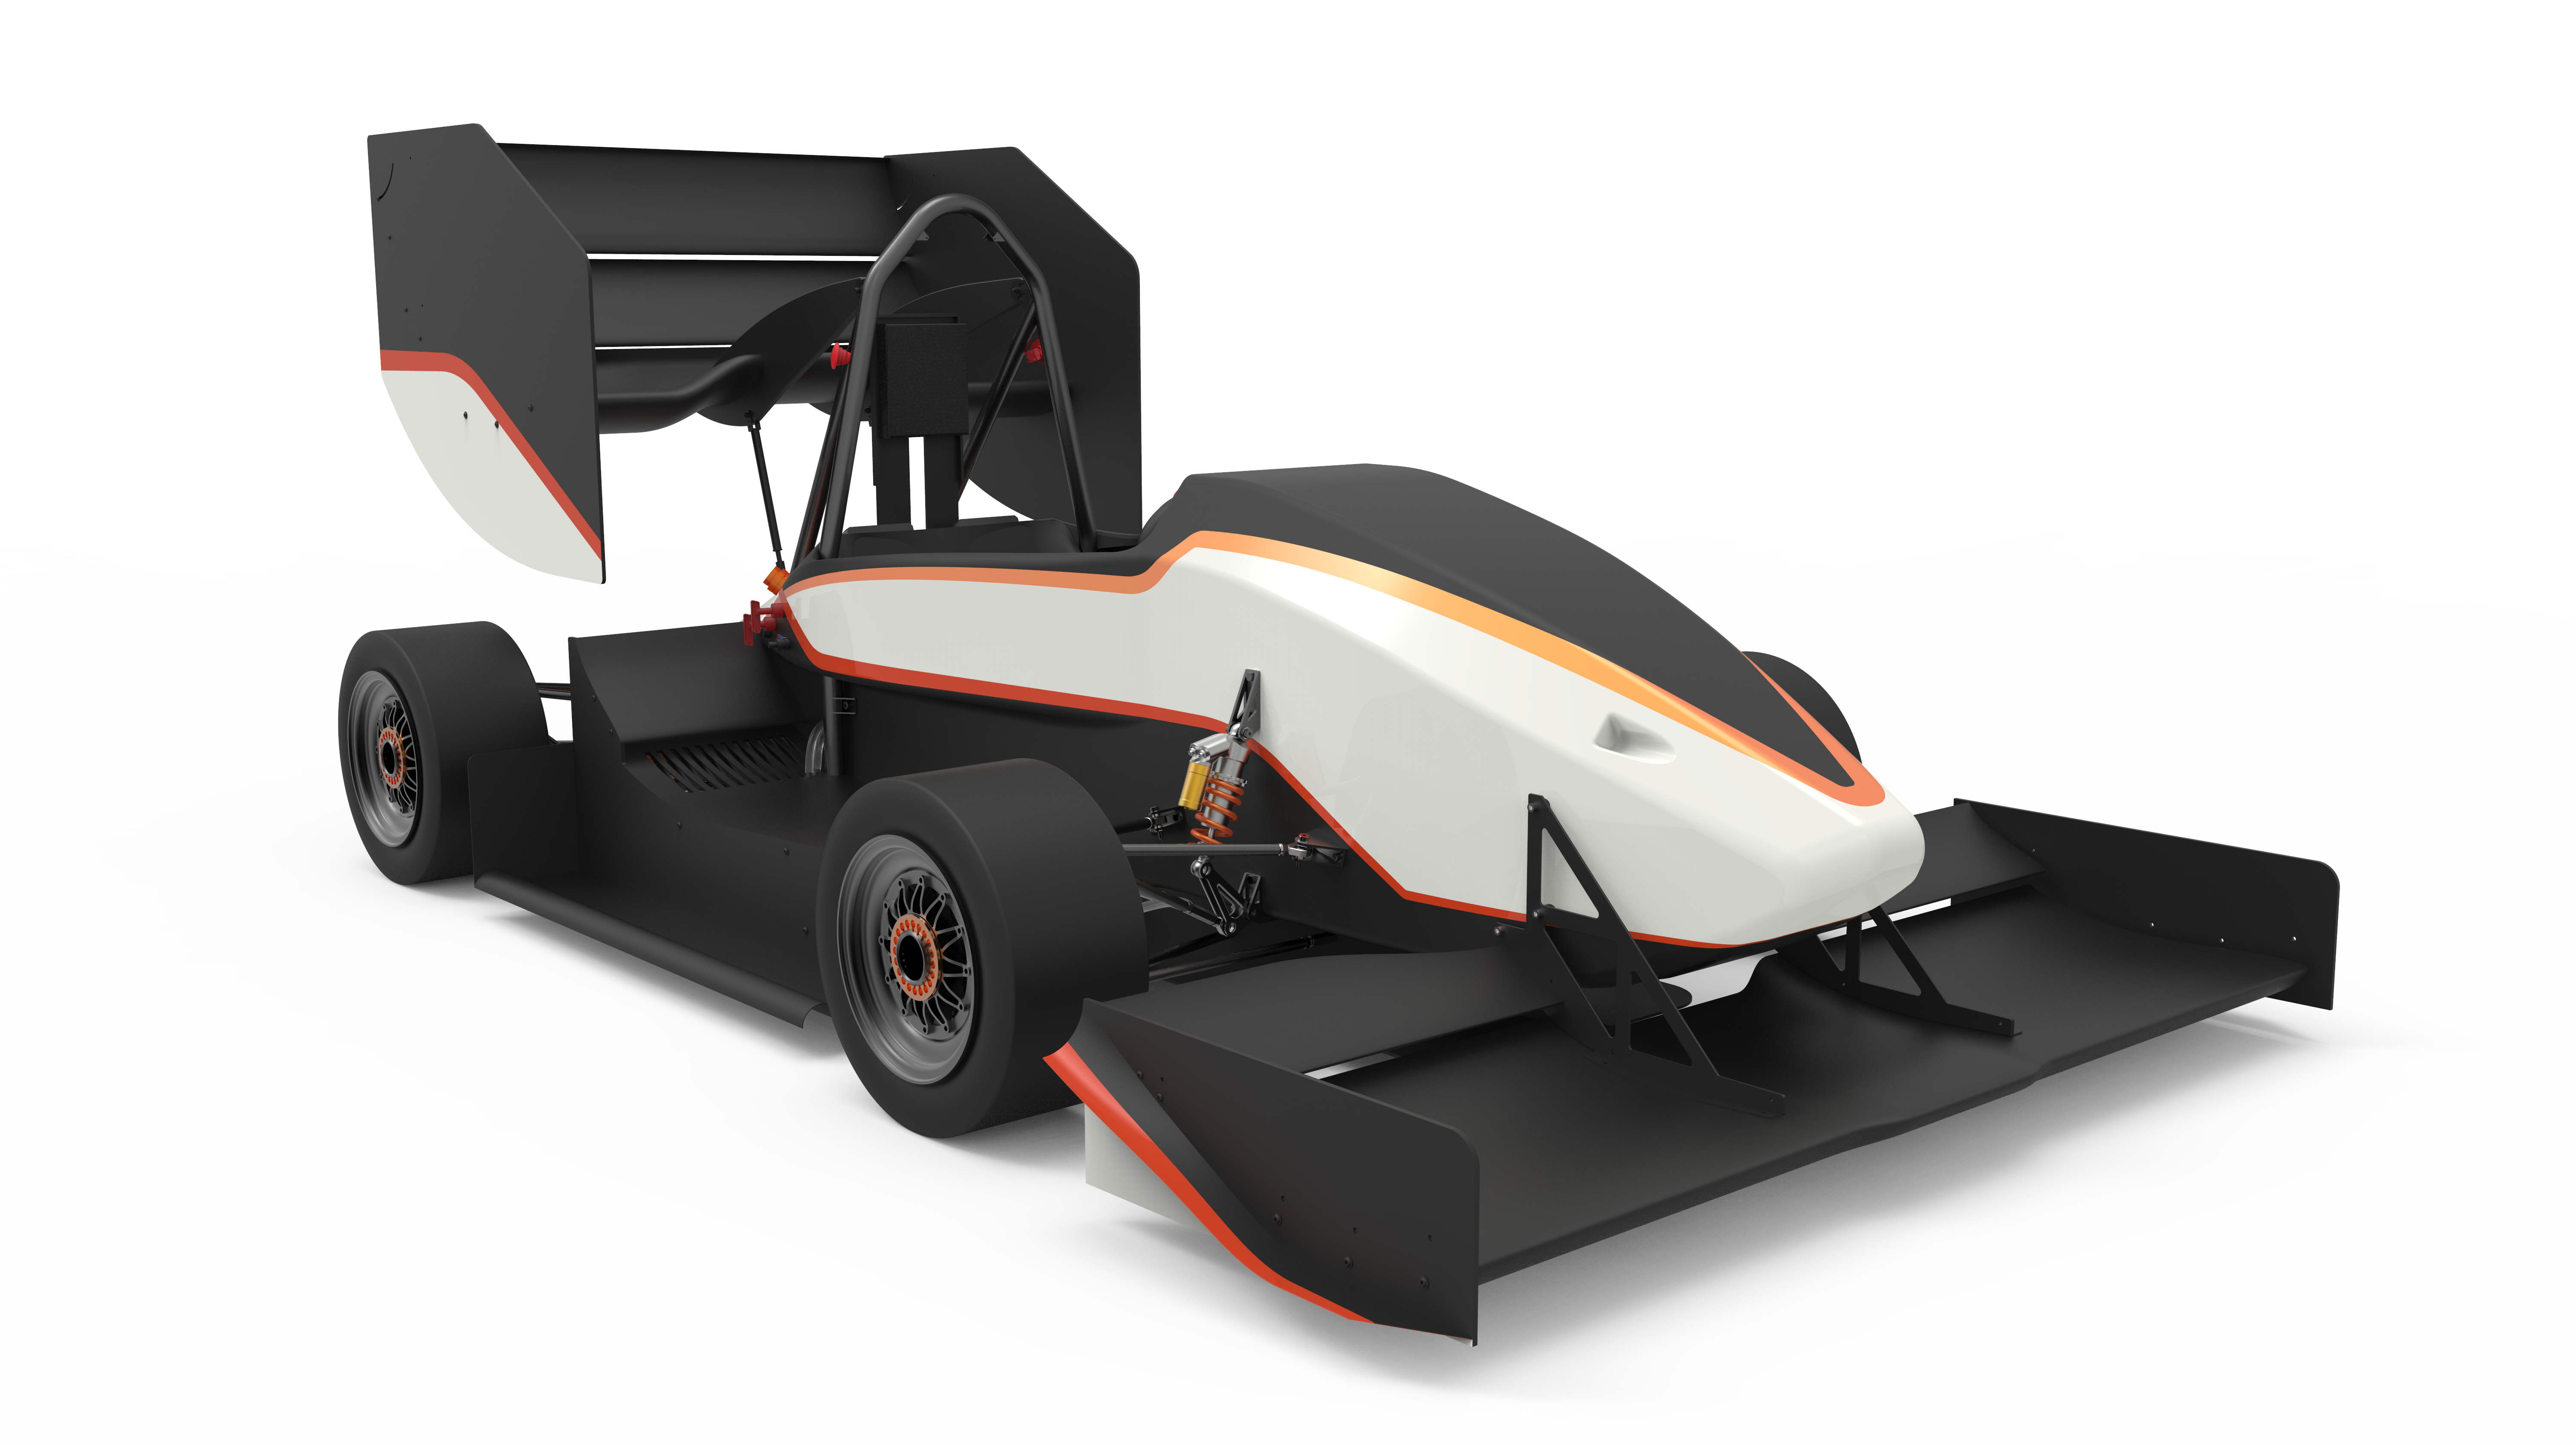
\includegraphics[width=\textwidth, trim={0cm 0cm 0cm 0cm}, clip]{./img/title-cover07.png}	
\vspace{.5cm}
%\vspace{1cm}
{\scshape\Large Czech Technical University in Prague\par}
%\vspace{1cm}
\vspace{.5cm}
{\LARGE eForce FEE Prague Formula\par}
%\vspace{1cm}
\vspace{.9cm}
{\LARGE E67\par}
%\vspace{1cm}
\vspace{.6cm}

\begin{table}[H]
	\centering
	%\flushright
	\begin{tabular}{rl}
		ESF responsible: &  \href{mailto:ondrej.sereda@eforce.cvut.cz}{Ondrej Sereda}  \\
		Team Captain: & Jan Kosina   \\
	\end{tabular}%
	\label{tab:title}%
\end{table}%

%{\large\itshape ESF responsible: Lukas Hostacny, email: lukas.hostacny@eforce.cvut.cz\\
%	Cc: Jan Kosina, email: jan.kosina@eforce.cvut.cz\par}


\vfill
	\end{titlepage}
%--------table of contens--------------------------------------
\pagenumbering{Roman}
%\sectionnumbering{Roman}
\setcounter{page}{1}

\addcontentsline{toc}{section}{\contentsname} \tableofcontents 
\newpage
 % List of Figures
	%\pagenumbering{roman} This is just Stupid
\addcontentsline{toc}{section}{I\quad\listfigurename} \listoffigures
\newpage
% List of Tables
\addcontentsline{toc}{section}{II \thinspace\thinspace \listtablename} \listoftables
\newpage
% List of Acronyms
\addcontentsline{toc}{section}{III List of Acronyms} \printglossary[type=\acronymtype,title=List of Acronyms]
\newpage

%\cleardoubleoddpage
\pagenumbering{arabic}
%\sectionnumbering{arabic}
%\setcounter{page}{1}
%-------ESF---------------------------------------------------
\section{System Overview}

Electrical systems of the car are divided into small blocks. The concept is to have all the systems distributed by 2 CAN buses (1st “CAN\_Powertrain” for systems crucial data to proper function, 2nd “CAN\_Aux” for all the other systems) and, if possible, all the signals transferred just by CAN bus. Baud rate is 500kbps and CAN is terminated in ECUP in front of car and in front motor controller by 120 Ohm resistor. There are in total 5 main control units – of course all the units are fully self-made (HW and FW).

\begin{itemize}
\item	ECUP (Electronic Control Unit Pedal)
This device measures brake pedal and acceleration pedal positions, implements safety algorithms regarding to rules about torque encoder check and outputs these values to the CAN bus as driver’s foot requests. It also monitors Shutdown Circuit – point BOTS. 

\item	VDCU – (Vehicle Dynamcs Control Unit)
This device reads driver’s foot requests, actual every wheel speed provided by ECUM and implements Traction Control Algorithms. The result is sent over private CAN bus to the MCF and MCR. 

\item	MC (Dual Motor Controller)
2 units in total – Front (MCF) and Rear (MCR). These units drives 4 motors in total, so every unit drives 2 motors. It provides speed of every wheel by actual RPM, temperatures and so on. Field Oriented Control is implemented with Resolvers as a position feedbacks.

\item	ECUF (Front + Dashboard)
Interaction with driver in cooperation with ECUS (Steering Wheel – LCD inside) by informing, warning and error LEDs, switches, rotary switches, push buttons. This is like a driver’s CAN bus console. 

\item	ECUB
Providing low voltage power distribution to all the control units and periphery (Li-Ion LV battery with BMS inside). This unit implements all the safety and control algorithms regarding to Shutdown Circuit rules. The main function is to latch SDC and evaluation of SDC interruption point. 

\item	ECUA
DC-DC converter, BMS, Pre-charge and AIR controlling is implemented. This unit also communicate with Charging Station.
There are other control and measuring systems not listed above, but systems listed are most important for safety and control. 

\end{itemize}

\iffalse
% table done
\begin{itemize}
\item Short description of the system’s concept 
\item Rough Schematic (blocks) showing all parts affected with the electrical systems and function of the tractive-system
\item No detailed wiring
\item Additionally, fill out the following table, replacing the values with your specifications:
\end{itemize}
\fi

\begin{table}[H]
	\centering
	\caption{General parameters}
	\begin{tabularx}{\textwidth}{|X|X|}
		\hline
		Maximum Tractive-system voltage: & 400 VDC  \\[\TableSize]
		\hline Nominal Tractive-system voltage: & 345.6 VDC\\[\TableSize]
		\hline
		Control-system voltage: & 24 VDC \\[\TableSize]
		\hline
		Accumulator configuration: & 96s9p \\[\TableSize]
		\hline
		Total Accumulator capacity: & 7.78 kWh\\[\TableSize]
		\hline
		Nominal HV Accumulator current: & 270 A \\[\TableSize]
		\hline
		Maximum HV Accumulator current: & 315 A \\[\TableSize]
		\hline
		HV accumulator cell type: & Lithium-Ion  \\[\TableSize]
		\hline
		LV Accumulator cell type: & Lithium-In \\[\TableSize]
		\hline
		Motor type: & PMSM with resolvers \\[\TableSize]
		\hline
		Number of motors: &  4, one per wheel \\[\TableSize]
		\hline
		Maximum combined motor power in kW & 109 \\[\TableSize]
		\hline
	\end{tabularx}%
	\label{tab:system-general}%
\end{table}%



\section{Electrical Systems}
% chybi obrazky a schema sdc a pozice v aute
\subsection{Shutdown Circuit}\label{subsec:SDC}
% This is copied from 2017 ESF and it is example of LaTex
% -------------------------------------------------------
% Ondřej Šereda 8.2.2018

\subsubsection{Description/concept}
\iffalse
Describe your concept of the shutdown circuit, the master switches, shut down buttons, brake over travel switch, etc.
Additionally, fill out the following table replacing the values with your specification and append additional switches from your setup:
\fi

Shutdown circuit (SDC) starts in \gls{ecup} unit, then goes through all \gls{sdc} elements in the car and ends in \gls{ecua}, which is placed inside the Accumulator Pack. In \gls{ecup} \gls{sdc} starts from \gls{lv} power +24V and ends in \gls{acp} by powering \gls{air} coils switching circuit (See \ref{fig:SDC-scheme}). The \gls{sdc} consists of 2 master switches, 3 shut-down buttons(SDB), the brake-over-travel-switch(\gls{bots}), the insulation monitoring device (\gls{imd}, the inertia switch, the brake system plausibility device(\gls{bspd}), interlocks in Motor Controllers and Accumulator Pack and the accumulator management system (\gls{ams}) and Front Wheel Interlock(FWIL). FWIL triggers shutdown circuit in case of front suspension failure(see doplnit figure kde je vyznaceny fwil). 

All of these crucial parts do not act through any power stage, but carry directly the \gls{air} current.

\todo[inline]{convert to full name refs}

\begin{figure}[H]
	\includegraphics[width=\textwidth, trim={2cm 3cm 2cm 2cm},clip]{./img/SDC-scheme.pdf}
	\caption{\gls{sdc} scheme.}
	\label{fig:SDC-scheme}
\end{figure}

\begin{table}[H]
	\caption{List of switches in the shutdown circuit}
	\centering
	\begin{tabu}{|X|l|}
		\hline Part  & Function \\
		\hline Main Switch (for control and tractive-system; CSMS, TSMS) & Normally open \\
		\hline Brake over travel switch (BOTS) & Normally closed \\
		\hline Shutdown buttons (SDB) & Normally closed \\
		\hline Insulation Monitoring Device (IMD) & Normally open \\
		\hline Battery Management System (BMS) & Normally open \\
		\hline Inertia Switch & Normally closed \\
		\hline Interlocks & Closed when circuits are connected \\
		\hline Brake System Plausibility Device & Normally Open \\
		\hline
	\end{tabu}%
	\label{tab:SDCswitch}%
\end{table}%
\todo[inline]{add refs}

\paragraph{Monitoring SDC}
Every part of \gls{sdc} is monitored by specific \gls{ecu} in order to identify disconnected element. \gls{bots} is measured by \gls{ecup}, SDB-center  and Inertia switch are measured by \gls{ecuf} , interlocks in \glspl{mc} (\gls{fwil}) are measured by \glspl{mc}, Interlock in Accumulator Pack is measured by \gls{ecua}  and finally SDB-right, SDB-left and \gls{tsms} are measured by \gls{ecub}. Every piece of information regarding the state of closure \gls{sdc} are running between ECU´s by \gls{can}. 

We designed \gls{sdc} to be ‘single wire’ alike and distanced it from the system as much as it was possible. In order to remain \gls{sdc} as a stand-alone wire we used optocouplers for main points of \gls{sdc}. Optocouplers are connected in such a way, that they become active only in case of nonzero voltage occurance at a certain point of \gls{sdc}.

\Gls{ecub} is last part of \gls{sdc} before \gls{tsms}. If a state of error on \gls{sdc} is detected \gls{ecub} latches the off-state of \gls{sdc} to stay off. If the occurred error is non-critical, it allows pilot to re-enter the TSON state. If monitored error is critical (such as \gls{imd} etc.), it notes the error to the memory-storage and does not allow \gls{sdc} to become active until appropriate steps are taken.

\paragraph{Master Switch}
We use Autolec Mini-Master battery cut-out switches with continuous current rating 100A, shown on \ref{fig:SDC-TSMS}.
\begin{figure}[H]
	\centering
	\includegraphics[width=.5\textwidth]{./img/SDC-TSMS.jpg}
	\caption{TSMS.}
	\label{fig:SDC-TSMS}
\end{figure}

\paragraph{Shutdown Switch}
We use OMRON A165E shutdown buttons, which have 3A current rating at 30VDC.

On the cockpit it is OMRON A165E-LS, shown on \ref{fig:SDC-A165E-LS}.
\begin{figure}[H]
	\centering
	\includegraphics[width=.5\textwidth]{./img/SDC-A165E-LS.pdf}
	\caption{Cockpit SDB.}
	\label{fig:SDC-A165E-LS}
\end{figure}

On the left and on the right sides there are OMRON A165E-LM buttons, shown on \ref{fig:SDC-A165E-LM}.
\begin{figure}[H]
	\centering
	\includegraphics[width=.5\textwidth]{./img/SDC-A165E-LM.pdf}
	\caption{SDB left and right.}
	\label{fig:SDC-A165E-LM}
\end{figure}

\paragraph{Brake Over Travel Switch}
It is type A165E-M, current raging 3A, shown on \ref{fig:SDC-A165E-M}
\begin{figure}[H]
	\centering
	\includegraphics[width=.5\textwidth]{./img/SDC-A165E-M.pdf}
	\caption{Brake over travel switch.}
	\label{fig:SDC-A165E-M}
\end{figure}


\subsubsection{Wiring / additional circuitry}
\iffalse
Describe wiring and additional circuitry, show extra schematics for example if additional transistors etc. are used, also describe the function of additional circuitry and make good use of figures.
Additionally, fill out and add information to the following table:
\fi

If connector is used to connect \gls{sdc} between control units, disconnecting any of them results in opening \gls{sdc} and therefore opening \glspl{air} as well. In other words the \gls{sdc} directly carries the current driving the accumulator isolation relays(\glspl{air}). All circuits that are part of the shutdown circuit have been designed in a way, that, when in disconnected state, they remove the current controlling the \glspl{air}.

The cross-section of Shutdown System wire is AWG22. Block wiring scheme shown on \ref{fig:SDC-schematic}.\\

\begin{figure}[H]
	\centering
	\includegraphics[width=\textwidth,trim={4cm 8cm 5cm 3cm}, clip]{./img/SDC-monitoring.pdf}
	\caption{Example of used \gls{sdc} monitoring method with optocouplers.}
	\label{fig:SDC-schematic}
\end{figure}

As shown, 4.7 k$\Omega$ resistors are used to limit current through optocoupler. With 24 V supply that makes 15.2 mA per optocoupler. We used 8 optocouplers: $12*15.2= 182.4$ mA.
% Table generated by Excel2LaTeX from sheet 'List1'
\begin{table}[H]
	\centering
	\caption{Wiring – Shutdown circuit}
	\begin{tabu}{|X|X|}
		\hline
		Total Number of \glspl{air}: & 2 \\
		\hline
		Current per \gls{air}: & 70 mA \\
		\hline
		Additional parts consumption within the shutdown circuit: & 182.4 mA \\
		\hline
		Total current: & 322.4 mA \\
		\hline
		Cross sectional area of the wiring used: & 0.322 mm$^2$ (AWG22) \\
		\hline
	\end{tabu}%
	\label{tab:SDC-Wiring}%
\end{table}%


\subsubsection{Position in car}
\iffalse Provide CAD-renderings showing the relevant parts. Mark the parts in the renderings, if necessary. \fi
\begin{figure}[H]
	\includegraphics[width=\textwidth]{./img/car-pos.jpg}
	\caption{Inertia switch, SDB Left, Right and Cockpit, \gls{tsms}, \gls{glvms}, HVD, Measure points.}
	\label{fig:SDC-positionInCar}
\end{figure}


\subsection{IMD}
% chybi tady reference na datasheet
\subsubsection{Description (type, operation parameters)}
\iffalse Describe the IMD used and use a table for the common operation parameters, like supply voltage, set point, etc. Also, describe how the IMD indicator light is wired, etc.
Additionally, fill out the following table replacing the values with your specification:\fi

We use A-ISOMETER® IR155-3203 Insulation monitoring device (IMD) for unearthed DC drive systems. Our maximum tractive voltage is 403.2 VDC. The rules require minimal insulation value between TS and GLVS 500 Ohm/V. Minimal resistance value for our car is 408*500 = 204 000 Ohm. This was set as request for manufacturer, and device was programmed in factory.
\begin{table}[H]
	\centering
	\caption{Parameters of the IMD}
	\begin{tabu}{|X|l|}
	 \hline	Supply voltage range: & 10..36VDC \\
	 \hline	Supply voltage & 24VDC \\
	 \hline	Environmental temperature range: & -40..105°C \\
	 \hline	Selftest interval: & Always at startup, then every 5 minutes \\
	 \hline	High voltage range: & DC 0..1000V \\
	 \hline	Set response value: & 204kΩ (500Ω/Volt) \\
	 \hline	Max. operation current: & 150mA \\
	 \hline	Approximate time to shut down at 50\% of the response value: & 20s \\
	  \hline
	\end{tabu}%
	\label{tab:IMD}%
\end{table}%

\subsubsection{Wiring/cables/connectors/}
 Describe wiring, show schematics, describe connectors and cables used and show useful data regarding the wiring including wire gauge/temp/voltage rating and fuses protecting the wiring. 

Relay of Insulation Monitoring Device is electrically placed between MCF and relay for AMS measurement. Wiring is done using Raychem Spec44 wire, AWG 22, rated to 600V. Wiring is shown on \ref{fig:SDC-scheme}. IMD opens relay in case of fault. IMD have output for relay, so there is not necessary adding zero diode on output. HV input to IMD is connected in according to datasheet.

\subsubsection{Position in car}
% Provide CAD-renderings showing the relevant parts. Mark the parts in the rendering, if necessary

\begin{figure}[H]
	\centering
	\includegraphics[width=\textwidth,trim={0cm 0cm 0cm 0cm},clip]{./img/IMD-position.jpg}
	\caption{IMD position.}
	\label{fig:IMD-position}
\end{figure}
\label{sebsec:IMD}

\subsection{Inertia Switch} \label{subsec:InertiaSwitch}
% nefunguje odakzy
\subsubsection{Description (type, operation parameters)}
\iffalse Describe the Inertia Switch used and use a table for the common operation parameters, like supply voltage, temperature, etc.
Additionally, fill out the following table replacing the values with your specification: \fi

Inertia switch opens shutdown circuit in case of acceleration more than 6g. After acting the driver can reset this switch.
\begin{table}[H]
	\centering
	\caption{Parameters of the Inertia Switch}
	\begin{tabularx}{\textwidth}{|X|l|}
	\hline	Inertia Switch type: & Sensata 510FCS01-01 \\[\TableSize]
	\hline	Supply voltage range: & No supply needed \\[\TableSize]
	\hline	Supply voltage: & No supply needed \\[\TableSize]
	\hline	Environmental temperature range: & -30 $^\circ$ 120 $^\circ$C \\[\TableSize]
	\hline	Max. operation current: & 10 A \\[\TableSize]
	\hline	Trigger characteristics: & 6 g for 60 ms / 11 g for 15 ms \\[\TableSize]
	\hline
	\end{tabularx}%
	\label{tab:inertiaSwitch}%
\end{table}%


\subsubsection{Wiring/cables/connectors}
%Describe wiring, show schematics, describe connectors and cables used and show useful data regarding the wiring.

Inertia switch is electrically placed between Shutdown button center on dashboard and the Shutdown input to \gls{ecub}, where is connected right Shutdown button on main hoop. Inertia switch will be connected by FQCT connectors. Wiring of inertia switch is shown on \ref{fig:SDC-scheme}. Wiring of inertia switch is shown on \ref{fig:SDC-scheme}.
\subsubsection{Position in car}
%Provide CAD-renderings showing the relevant parts. Mark the parts in the rendering, if necessary.

Inertia switch is placed on the right side in the cockpit clearly shown in \ref{fig:SDC-positionInCar}.

\subsection{Brake Plausability Device} \label{subsec:BSPD}
% Responsible: Mark G.
% Author: Mark G.

\subsubsection{Description/additional circuitry}
% Describe how your electronic hardware brake plausibility system works (this is in addition to your ECU controlled brake plausibility software), provide tables with main operation parameters, and describe additional circuitry used to check or for an implausibility. Describe how the system reacts if an implausibility or error is detected.

\Gls{bspd} is represented by a \gls{pcb} with an on-board current transducer. It’s function is to monitor
power drawn from \gls{acp} and brake pedal pressure, and open \gls{sdc} in case both signals are above
allowed threshold for more than 0.5 seconds. Also, the event of disconnection of \gls{sdc} is latched,
thus it gets to reset only in case of the main power reset.


\begin{table}[H]
	\centering
	\caption{BSPD data}
	\begin{tabu}{|X|X|}
		\hline
		Brake sensor used: & Piezoresistive Pressure Transmitter PA-21Y / 100bar / 81691.1 \\
		\hline
		Brake sensor physical response value: & Voltage, 4.5V \\
		\hline
		Tractive system power sensor type & Current Transducer LEM HTFS 200-P \\
		\hline
		Tractive system sensor physical response value: & Voltage of 85 mV \\
		\hline
		Tractive System power sensor current threshold (5kW/Nominal \gls{ts} voltage): & 14 A \\
		\hline
		Supply voltages: & 5 V \\
		\hline
		Maximum supply currents: & 22 mA \\
		\hline
		Operating temperature: & -40 $^\circ$C to 105 $^\circ$C \\
		\hline
		Output used to control \glspl{air}: & Open a MOSFET in \gls{sdc} \\
		\hline
	\end{tabu}%
	\label{tab:bspd}%
\end{table}%

Complete datasheet: \ref{app:bspd_lem_datasheet}

\iffalse
\begin{figure}[H]
	\centering
	\includegraphics[width=\textwidth]{./img/bspd-position.jpg}
	\caption{\Gls{bspd} flowchart.}
	\label{fig:BSPD-flowchart}
\end{figure}\fi

\subsubsection{Schematic}
%Describe the wiring, show schematics including the circuit board, show data regarding the cables and connectors used
The \gls{bspd} \gls{pcb} is mounted on a \gls{hv} wire in such manner, that the \gls{hv} wire goes through the
current transducer. Current transducer provides analog voltage output of a value proportional to
actual current (resp. power) drawn from \gls{acp}. This voltage is amplified and is converted to two-state
logic levels voltage with the use of comparators. The value of “High” current signal logic level
is set to be at 5kW of power drawn from \gls{acp} (14A).

Brake state is measured in \gls{ecup}, converted with help of a comparator to two-state logic levels
voltage and is sent directly to \gls{bspd} via wiring.

Both logic signals are connected to NAND inputs. When both inputs are at “High” level, a
capacitor $C_1$ starts to charge through resistance $R_{16}$. When voltage on $C_1$ is higher than 2.5V, a
comparator $U_{1B}$ sends signal to open \gls{sdc}.

\begin{figure}[H]
	\centering
	\includegraphics[width=\textwidth]{./img/bspd-schematic.pdf}
	\caption{\gls{bspd} schematic sheet}
	\label{fig:BSPD-schematic}
\end{figure}

\subsubsection{Connection with shutdown circuit}
The connection to \gls{sdc} is provided by an NPN transistor $Q_2$ and a P-Channel MOSFET $Q_1$, that
are connected to act as a “normally-closed” switch in \gls{sdc} loop. Thus in case of a trip event $Q_1$
stops conducting current between Drain and Source. See \ref{fig:BSPD-schematic}.

This state is latched by a latch-circuit, that consists of two NAND gates.

\iffalse
\begin{figure}[H]
	\centering
	\includegraphics[width=\textwidth]{./img/bspd-position.jpg}
	\caption{\gls{bspd} connection with \gls{sdc}.}
	\label{fig:BSPD-conn}
\end{figure}\fi

\subsubsection{Position in car/mechanical fastening/mechanical connection}
%Provide CAD-renderings showing all relevant parts and discuss the mechanical connection of the sensors to the pedal assembly. Mark the parts in the rendering, if necessary.

BSPD is placed in Service Box, which connects high voltage harnesses from accumulator pack to motor controllers. The board containing BSPD circuit and current transducer is mounted to a wire.
\begin{figure}[H]
	\centering
	\includegraphics[width=\textwidth]{./img/ServiceBox-position.jpg}
	\caption{\gls{bspd} position}
	\label{fig:BSPD-position}
\end{figure}


\subsection{Reset / Latching for IMD and BMS} \label{subsec:Reset}
% Responsible: Kdokoliv
% ECUB scheme and circuitry, state machine and other
\subsubsection{Description/circuitry}
% Describe the concept and circuitry of the latching/reset system for a tripped IMD or AMS.  Describe the method for resetting the IMD and AMS.
The \gls{ams} and \gls{imd} error is latched in the \gls{ecua} circuitry. The \gls{sdc} is switched by Q$_2$ and Q$_3$ respectively. Both \gls{ams} and \gls{imd} states are positive logic (AMS\_OK and IMD\_OK), combined using th first U$_2$ gate. If either of the two signals goes to zero (\gls{imd} error or \gls{ams} error), the output of U$_2$ goes high. That triggers the latching circuit comprised of Q$_4$ and Q$_5$. Q$_4$ and Q$_5$ forms a classic thyristor structure, that can be reset only by a power cycle.  There is a few seconds delay introduced in the latch activation by U$_1$ and the RC timing network. This is to accommodate for the \gls{imd} and \gls{ams} self-test/start-up routines, when the AMS\_OK and IMD\_OK signals are not yet asserted. During this delay, the \gls{sdc} is forced open by the action of U$_4$. It is therefore not possible to start the car (\gls{sdc} open) during the self-test/start-up time, when the latch is disabled.
5 V power for this circuit is derived from the 24 V \gls{glvs}, after \gls{glvms}, using a linear regulator.


\subsubsection{Wiring/cables/connectors}
%Describe wiring, show schematics, describe connectors and cables used and show useful data regarding the wiring.  If not detailed in section 2.1, be sure to show how the device opens the shutdown circuit.
% SDC monitoring scheme
Whole latching circuit is implemented in \gls{ecua}.


\subsubsection{Position in car}
%Provide CAD-renderings showing the relevant parts. Mark the parts in the rendering, if necessary.
\Gls{imd} and \gls{ams} error latch is placed in \gls{ecua} on the back of car. See \ref{fig:ECUA}.

\begin{figure}[H]
	\centering
	\includegraphics[width=\textwidth]{./img/ECUA_imd_ams_latch.pdf}
	\caption{\Gls{ams} \gls{imd} latch schematic.}
	\label{}
\end{figure}

\subsection{Shutdown System Interlocks}\label{subsec:SDCInterlocks}
% figures and renderings 
%Responsible: Jano
\subsubsection{Description/circuitry}
\iffalse Describe the concept and circuitry of the Shutdown System Interlocks.
Note: Interlocks are circuits used to open the shutdown circuit if a connector is disconnected or enclosure is opened.  This is not the entire shutdown circuit.\fi

We have interlocks in ACP HV connector (connector HV\_A), Motor controller HV inputs and outputs, HV connector in Service box, HVD and in the LV connectors from MC´s (MCR and MCF) to motor (connectors M1, M2, M3 and M4). 

In all HV connectors and LV connectors to motors we have a loop, that in case of disconnection from car opens Shutdown circuit.

\subsubsection{Wiring/cables/connectors}
%Describe wiring, show schematics, describe connectors and cables used and show useful data regarding the wiring.

Scheme of entire Shutdown circuit can be found at \ref{fig:SDC-scheme}.

\subsubsection{Position in car}
%Provide CAD-renderings showing the relevant parts. Mark the parts in the rendering, if necessary.
HVD is clearly shown above in \ref{fig:SDC-positionInCar}. For Service box position see \ref{fig:ServiceBox-position}

Last interlock is in Accumulator Pack HV Connector shown in ACP HV Connector.

\subsection{Tractive System Active Light}\label{subsec:TSAL}
% Responsible: Janko, Emil, Manek
%ECUB, schemata tsal + schema v ecub + schemes + renders
\subsubsection{Description / circuitry}
% Describe the tractive system active light and additional circuitry. Additionally, fill out the table:

The \gls{tsal} is a distributed system consisting of the following components:
\begin{itemize}
\item Tractive System Active Light mounted on main hoop
\item \gls{tsal} logic \& power circuitry (located in \gls{ecub}; LV only)
\item DC-DC converter to power the \gls{tsal} in case of charged TS but unpowered \gls{glvs} (located in the \gls{acp}; has a \gls{hv} side and a LV side)
\end{itemize}

\paragraph{Tractive System Active Light}

The \gls{tsal} proper is connected with 2 wires. When voltage of 24 V is applied, the \gls{tsal} lights up either in green or red color depending on the polarity.

\begin{figure}[H]
	\centering
	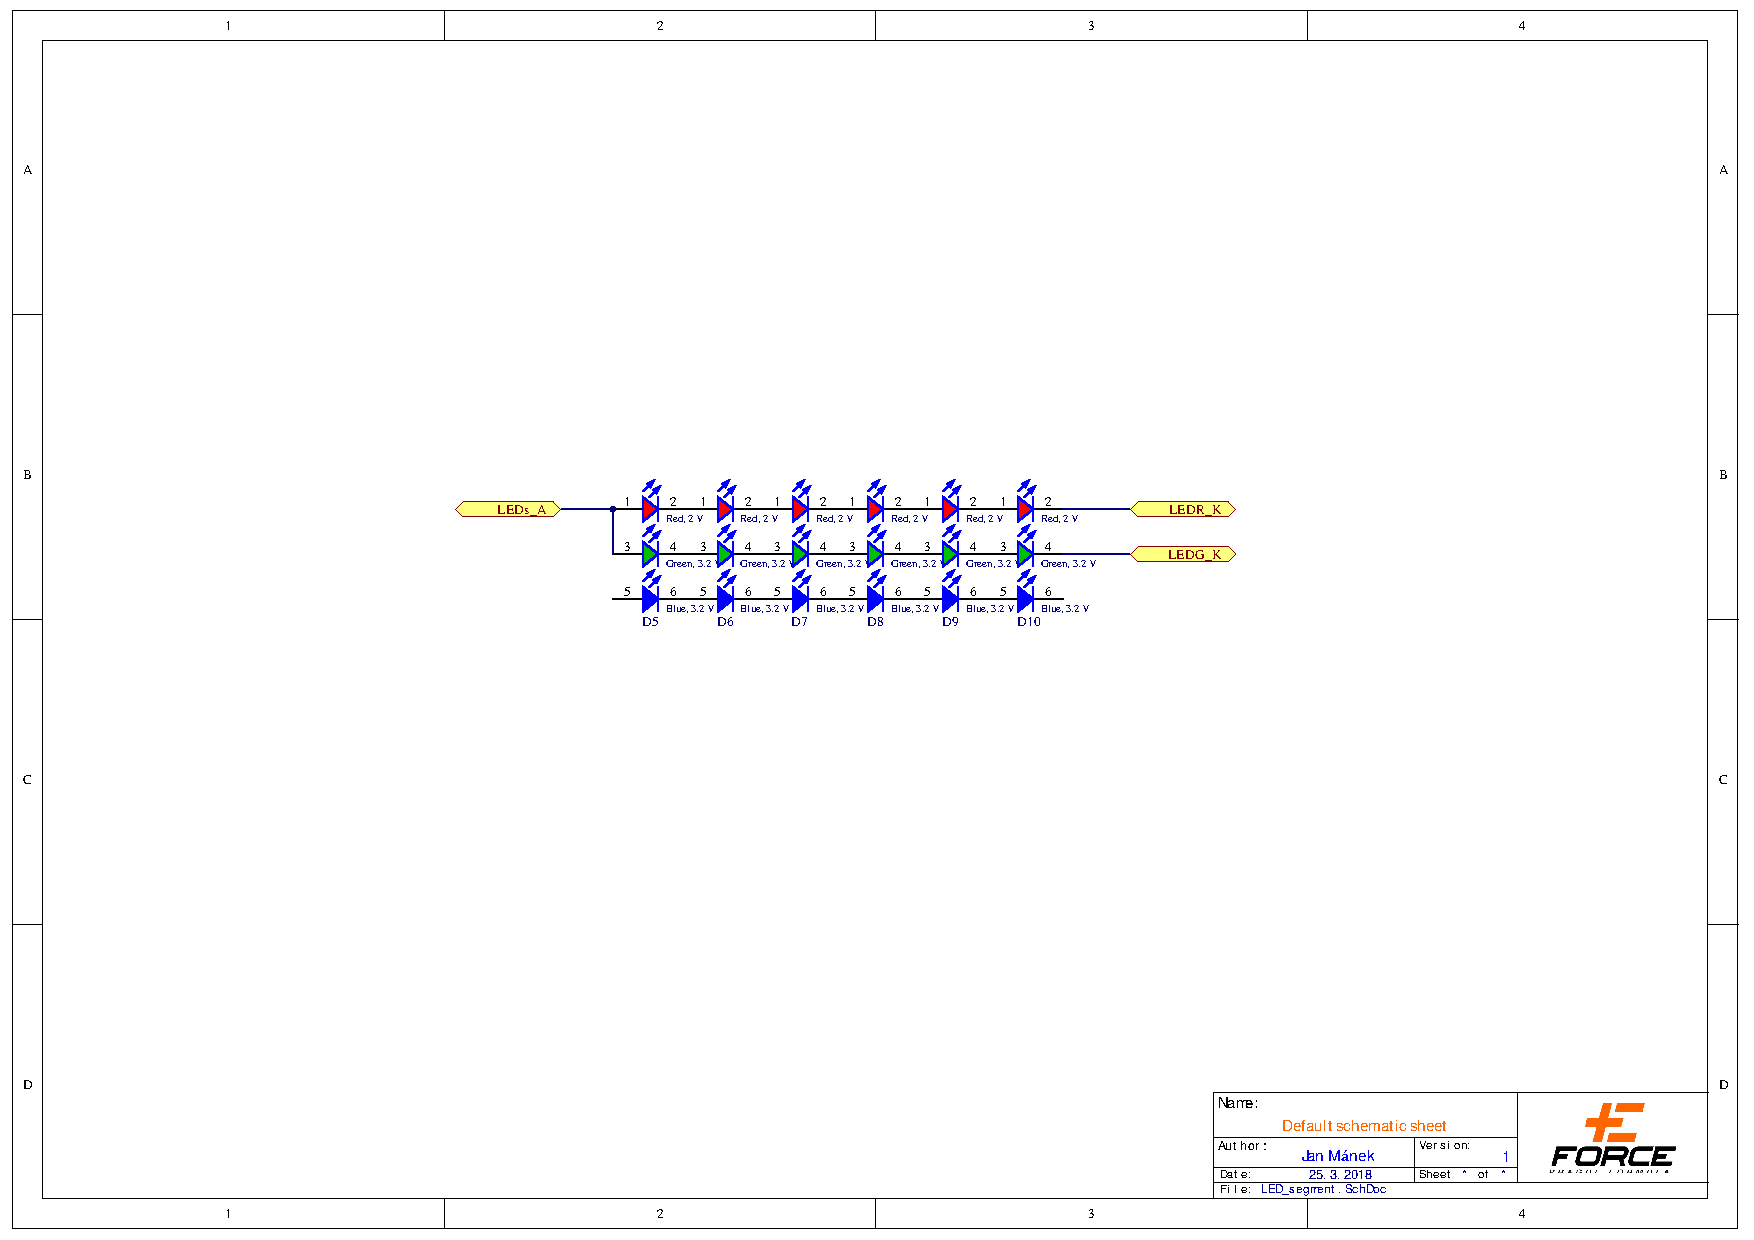
\includegraphics[width=\textwidth,trim={6cm 10cm 6cm 7cm},clip]{./img/TSAL-schematic.pdf}
	\caption{TSAL schematic.}
	\label{fig:TSAL-schematic}
\end{figure}


\begin{table}[H]
	\centering
	\caption{Parameters of the TSAL}
	\begin{tabularx}{\textwidth}{|X|X|}
		\hline
		Supply voltage: & +/- 24VDC \\[\TableSize]
		\hline
		Max. operational current: & 300mA \\[\TableSize]
		\hline
		Lamp type & Bi-color LED \\[\TableSize]
		\hline
		Power consumption: & 7.2 W \\[\TableSize]
		\hline
		Brightness & 124 Lumen (red), 29 Lumen (green) \\[\TableSize]
		\hline
		Frequency: & 3.96Hz \\[\TableSize]
		\hline
		Size (length x height x width): & 128mm x 20mm x 32mm \\[\TableSize]
		\hline
	\end{tabularx}%
	\label{tab:TSAL}%
\end{table}%

\paragraph{TSAL logic \& power circuitry}

To power the \gls{tsal}, a voltage of approximately 24 V is needed. This can be supplied either by the \gls{glvs}, or by a charged Tractive System by means of an isolated DC-DC converter.

A 5V rail is also generated to control all TSAL-related logic. (\ref{fig:TSAL-ECUB-5V})

\begin{figure}[H]
	\centering
	\includegraphics[width=0.6\textwidth]{./img/TSAL-ECUB-5V.png}
	\caption[Powering of the TSAL]{Powering of the \gls{tsal}. \gls{glvs} power is denoted \texttt{VCC}.}
	\label{fig:TSAL-ECUB-5V}
\end{figure}

Discrete logic is used for selecting the light colour. (\ref{fig:TSAL-logic})

\begin{figure}[H]
	\centering
	\includegraphics[width=\textwidth]{./img/TSAL-logic.png}
	\caption[TSAL enable logic]{TSAL enable logic. The signals \texttt{TSAL-RED} and \texttt{TSAL-GREEN} are always complementary.}
	\label{fig:TSAL-logic}
\end{figure}

A 555 IC is used to generate the required frequency which is used to modulate the power output. (\ref{fig:TSAL-555})

\begin{figure}[H]
	\centering
	\includegraphics[width=0.6\textwidth]{./img/TSAL-555.png}
	\caption[TSAL frequency generator]{\gls{tsal} frequency generator. When a green light is desired (\gls{glvs} active, \gls{ts} not charged), oscillation is suppressed and the output \texttt{TSAL-PWM-IN} is a constant logical '1'.}
	\label{fig:TSAL-555}
\end{figure}

Finally, a H-bridge is used to drive the proper power outputs with switchable polarity. (\ref{fig:TSAL-H-bridge})

\begin{figure}[H]
	\centering
	\includegraphics[width=0.5\textwidth]{./img/TSAL-H-bridge.png}
	\caption{\gls{tsal} power H-bridge}
	\label{fig:TSAL-H-bridge}
\end{figure}

\ref{fig:TSAL-logic-table} summarizes operation of the \gls{tsal}.

\begin{table}[H]
	\centering
	\caption{TSAL logic table}
	\begin{tabularx}{\textwidth}{|X|X|X|X|X|}
		\hline
		\textbf{Tractive System state} & \textbf{GLVS state} & \textbf{TSAL powered from} & \textbf{TSAL polarity} & \textbf{TSAL waveform} \\
		\hline
		not charged & off & not powered & -- & -- \\
		\hline
		not charged & on & 24V GLVS & negative (green) & Always-on \\
		\hline
		precharging & on & 24V GLVS & positive (red) & Square wave, 3.96Hz, 50\% duty cycle \\
		\hline
		charged & don't care & TS & positive (red) & Square wave, 3.96Hz, 50\% duty cycle \\
		\hline
	\end{tabularx}%
	\label{fig:TSAL-logic-table}
\end{table}%

\paragraph{DC-DC converter}

To ensure that the \gls{tsal} continues to operate even after disabling \gls{glvs}, the following circuit is used:

\begin{figure}[H]
	\centering
	\includegraphics[width=\textwidth]{./img/ECUA_TSAL_POWER.pdf}
	\caption{TSAL HV part schematic.}
	\label{fig:TSAL-HV}
\end{figure}

\paragraph{Explanation of TSAL circuit}
\Gls{tsal} \gls{hv} part schematic \ref{fig:TSAL-HV} is directly connected to the output \gls{hv} pins of \gls{acp}. The circuit is designed with STMicroelectronics chip VIPer53 (\ref{app:viper_datasheet}). The circuit functions as a fly-back DC/DC converter, directly supplying the \gls{tsal}. The converter starts operating at about 40 V, but the output to \gls{tsal} is switched through $Q_2$ only when the HV voltage is more than 60 V. That is ensured using D4, which together with $Q_1$ works as a precise 60 V comparator with a little introduced hysteresis.

The \gls{acp} indication led is powered from the primary side of the transformer, from the VIPER53's own supply voltage.
In case of any of the \glspl{air} closed, or the pre-charge relay contact being detected closed (please see \ref{subsec:precharge}  for details), the \gls{tsal} is supplied from the \gls{glvs} 24 V system, through Q$_2$. The "relay closed" signals from both \glspl{air} and the pre-charge relay are OR-ed together using hardwired logic (i.e. 74LVC2G32).

%schema z backu
\subsubsection{Wiring/cables/connectors}
\iffalse Describe wiring, show schematics, describe connectors and cables used and show useful data regarding the wiring.  Include gauge, voltage and temperature rating of wiring used and any fuses or other overcurrent protection used.\fi

LEDs are supplied from \gls{ecub} (by Harness\_D by connector D1) by 2-wire low voltage cable (\ref{fig:TSAL-wiring}).

\begin{figure}[H]
	\centering
	\includegraphics[width=\textwidth,]{./img/tsal-wiring.jpg}
	\caption{Wiring \gls{tsal} from \gls{ecub}}
	\label{fig:TSAL-wiring}
\end{figure}

\subsubsection{Position in car}
%Provide CAD-renderings showing the relevant parts. Mark the parts in the rendering, if necessary.
\gls{tsal} is placed under the main roll hoop, see \ref{fig:TSAL-position}

\begin{figure}[H]
	\centering
	\includegraphics[width=\textwidth,trim={3cm 11cm 2cm 1cm},clip]{./img/tsal-position.pdf}
	\caption{\Gls{tsal} position.}
	\label{fig:TSAL-position}
\end{figure}

\begin{figure}[H]
	\centering
	\includegraphics[width=\textwidth]{./img/ECUB_POSITION.jpg}
	\caption{\gls{bspd} schematic sheet}
	\label{fig:ecub_position}
\end{figure}


\subsection{Measurement points}\label{subsec:MeasurementPoints}
%Responsible: Janko
%schemata
\subsubsection{Description}
%Describe the housing used and how it can be accessed, etc.  Describe how the measurement points protected/covered when not in use and how the electrical connections on the back of the measurement points are protected when the measurement points are being used.

High voltage measurement points (HVMP) are placed in the Service box. When not in use, they are covered with protective cups made from silicone rubber. From backside they are protected by sealed Service box all the time.
\subsubsection{Wiring, connectors, cables}
%Describe wiring, show schematics, and describe connectors and cables used and show useful data regarding the wiring.  Include details on the protection resistor including resistance, voltage and power rating.

They are connected to ECUB (by Harness\_G with connector G1). In ECUB is TSAL switch circuit and discharge circuit is in ECUM (ECUM is connected to ECUB by Harness\_E – connectors are E1 from ECUB and E2 into ECUM Rear).
HVMP wires will be connected to the board in ECUB box, where is TSAL switch circuit, discharge circuit and 2 resistors 15k 1W (R1, R2) for HVMP. Value of this resistor can be measured from measuring points by multimeter with switched TSMS off.

\subsubsection{Position in car}
%Provide CAD-renderings showing the relevant parts. Mark the parts in the rendering, if necessary.

Measure points are placed on panel next to Master switches and HVD, see \ref{fig:SDC-positionInCar}.

\subsection{Pre-Charge circuitry}\label{subsec:PrechargeCircuitry}
%Responsible: JSi
%ECUA
\subsubsection{Description}

\begin{figure}[H]
	\centering
	\includegraphics[width=\textwidth,clip]{./img/ECUA_AIRS.pdf}
	\caption{TS pre-charge circuit and switching schematic.}
	\label{fig:precharge_sch}
\end{figure}

Principial block schematic of the TS switching circuit (including pre-charge) is in the \ref{fig:precharge_sch}. Pre-charge circuit is part of and controlled by ECUA. Pre-charge circuit is comprised of a relay RE3 and two series connected power resistors R1 and R2. 

Both resistors are located on a heat-sink, that is shared with the DC/DC converters, mentioned in section 9.2 of this document. The task of the heat-sink is to enhance the power overload capacity of the pre-charge resistors during the initial overload during the beginning of the charging curve, shown in \ref{fig:precharge_voltage_time}.

\begin{figure}
	\begin{tikzpicture}
		\begin{axis}[
			use units,
			x unit=s,
			y unit=V,
			xlabel=time,
			ylabel=volatge,
			width=0.9\textwidth,
			height=0.5\textwidth,
			grid=major,
			xmin=0,
			ymin=0,
			xmax=10
			]
		\addplot[red, smooth] table[
			x=time,
			y=voltage,
			col sep=comma
			] {./data/TS_precharge.csv}; 
		\end{axis}
		\end{tikzpicture}
		\caption{Pre-charge voltage in time.}
	\label{fig:precharge_voltage_time}
\end{figure}

The formula describing \ref{fig:precharge_voltage_time} is:

\begin{equation}
	I_{d}=1-e^{(\frac{-t}{R*C})}
	\label{eq:precharge_voltage}
\end{equation}

\begin{figure}
	\begin{tikzpicture}
	\begin{axis}[
	use units,
	x unit=s,
	y unit=A,
	xlabel=time,
	ylabel=current,
	width=0.9\textwidth,
	height=0.5\textwidth,
	grid=major,
	xmin=0,
	ymin=0,
	xmax=10
	]
	\addplot[red, smooth] table[
	x=time,
	y=current,
	col sep=comma
	] {./data/TS_precharge.csv}; 
	\end{axis}
	\end{tikzpicture}
	\caption{Precharge current in time.}
	\label{fig:precharge_current_time}
\end{figure}


The formula describing \ref{fig:precharge_current_time} is:

\begin{equation}
	I_{d}=\frac{V_{c}}{R_{d}}	
\end{equation}

\begin{equation}
	I_{d}=\frac{V_{s}*(1-e^{(\frac{-t}{R*C})})}{R_{d}}
	\label{eq:precharge_current}
\end{equation}


Both wirewound power resistors, ARCOL HS25 series, have 250 $\Omega$, 25 W continuous rating, DATASHEET.

All three TS relays RE$_1$ to RE$_3$ coils are powered directly from the SDC end.

After the SDC circuit is complete and closed (voltage present at SDC END), the precharge sequence is begun by closing AIR I (RE1). Then a pre-charge relay RE3 is closed. Voltage both on the ACP and output side is monitored using the measurement block, through the $HVR_1$ and HVR$_2$ resistor dividers. After the voltage difference is low enough (determined by ECUA software), AIR II (RE2) is closed, RE3 can be released.

Safety of the AIR switching and pre-charging is done by the ECUA firmware, that evaluates all possible circuit states. Voltages are measured on the ACP and ACP output sides using the measurement block, AIR physical states are observed using the auxiliary contacts and the pre-charge relay physical contact state is observed using the principle in the \ref{fig:precharge_sch}, via the diode D$_1$. The PCH\_SNS signal is pulled low whenever the pre-charge relay RE3 contact is closed.

Several safety precautions are implemented, on top of the Rules. First of such implemented protections is HW non-programmable voltage difference sensing across the pre-charge relay or AIR II respectively. This is done using the two voltage measurement dividers HVR$_1$ and HVR$_2$. There is a differential amplifier and comparator, that prevents closing both AIR relays in case of high voltage difference across the AIR II. 

Diodes D2 and D3 serve to block current flow to the output in case of AIR I is open. This specific topology was chosen to be able to measure the difference voltage across the AIR II utilizing only analog non-programmable circuitry.

Second precaution is a HW circuit limiting the maximum pre-charge relay closed time, and assuring a minimum off time for the pre-charge resistor to cool off. This circuit is a non-programmable one, realized using a discrete logic. In case of a pre-charge time-out or failure (voltages not equalized), AIR I (the Tyco Kilovac EV200 ODKAZNAKONECUZJETAMDATASHEET) is disconnected always first (instead of the pre-charge relay RE3), because the AIR does have the required DC breaking capacity.

Additional precision ACP voltage measurement is taken using the HVR$_3$ sense divider, as this measurement is not influenced by the forward voltage drops of diodes D$_2$ to D$_5$. This measurement together with the measured ACP current serves to calculate power drawn from the ACP. This measurement is then presented on the CAN bus for other car ECUs, for example to estimate the SOC, instantenous power, etc.  

The TS voltage sensing dividers HVR1, HVR2 and HVR3 are realized with a high voltage 3500 V rated resistors from Vishay, HVR37 series (DATASHEEEEET). All dividers use 10 Mohm resistors as the top side of the divider. All diodes D1 to D5 are SM4007 (DATASHEET) or equivalent type, 1000 V rated. The blocking voltage is therefore sufficient to safely withstand the maximum ACP voltage of 400 V.

\paragraph{Pre-charge safety on ECUA}
Except from what rules require we implemented several safety precautions. In case, that SDC error doesn’t occur and driver pushed TS ON button following safety precautions are taken to prevent switching AIR in case of problem that has not yet been detected.

First one is completely non-programmable protection against switching voltage difference by AIR. It uses voltage measurement and then comparators and logic to disable microcontroller decision in case of SW error.
Second one is measuring all states and voltages by microcontroller on ECUA which can determinate error before non-programmable protection would have to act.

Third (time-out) protection is used when everything seems to be OK, but the charging is too slow – caused by too high pre-charge resistance (any of pre-charge resistors fails), or some leakage of charge in capacitor or any other possible error occurs. If voltage difference is not equaled in time less them 2seconds, the ECUA stops pre-charge and waits 5 seconds before trying again. (In order to not overpower resistors.) If number of attempts to pre-charge is in this state higher then 8, something is clearly wrong and ECUA opens SDC and indicates error. Sending message about error and sets car into not-ready state.

\subsubsection{Wiring, cables, current calculations, connectors}
Describe wiring, show schematics, describe connectors and cables used and show useful data regarding the wiring.

%\item Give a plot “Percentage of Maximum Voltage” vs. time
%\item Give a plot Current vs. time 
%\item For each plot, give the basic formula describing the plots


Additionally, fill out the tables:

\begin{table}[H]
	\centering
	\caption{General data of the pre-charge resistor}
	\begin{tabularx}{\textwidth}{|X|X|}
		\hline
		Resistor Type: & \\[\TableSize]
		\hline
		Resistance: & \\[\TableSize]
		\hline
		Continuous power rating: & \\[\TableSize]
		\hline
		Overload power rating (1 sec): &  \\[\TableSize]
		\hline
		Overload power rating (5 sec): &  \\[\TableSize]
		\hline
		Overload power rating (15 sec): &  \\[\TableSize]
		\hline
		Voltage rating: & \\[\TableSize]
		\hline
		Cross-sectional area of the wire used: & \\[\TableSize]
		\hline
	\end{tabularx}%
	\label{tab:precharge-general}%
\end{table}%

\begin{table}[H]
	\centering
	\caption{General data of the pre-charge relay}
	\begin{tabularx}{\textwidth}{|X|X|}
		\hline
		Relay Type: & \\[\TableSize]
		\hline
		Contact arrangment: &  \\[\TableSize]
		\hline
		Continuous DC current:  & \\[\TableSize]
		\hline
		Voltage rating  & \\[\TableSize]
		\hline
		Nominal Coil Voltage: &  \\[\TableSize]
		\hline
		FET type: &  \\[\TableSize]
		\hline
		Maximum Drain-Source Current: &  \\[\TableSize]
		\hline
		Drain-Source Breakdown Voltage: &  \\[\TableSize]
		\hline
		On Charasteristics Gate Threshold Voltage: & \\[\TableSize]
		\hline
		Cross-sectional area of the wire used: & \\[\TableSize]
		\hline
	\end{tabularx}%
	\label{tab:precharge-relay}%
\end{table}%

\subsubsection{Position in car}
Provide CAD-renderings showing all relevant parts. Mark the parts in the rendering, if necessary.

\subsection{Discharge circuitry}\label{subsec:DischargeCircuitry}
%ECUB
\input{./tex/DischargeCircuitry.tex}

\subsection{HV Disconect (HVD)}\label{subsec:HVD}
%Responsible: Jano
%Datasheety, rendery
\subsubsection{Description}
%Describe your concept of the HVD and how it can be operated.

A circular connector ASHD 0 22-24320 S N + ASHD 6 22-24320 P N is used as HVD. By disconnecting HVD a positive pole of Tractive System is quickly disconnected. Disconnection is done by turning the plug left, this motion is clearly hinted by a label. By turning left the lever system in connector disconnect pins and release plug. There are sockets used in the receptacle rather than pins, therefore no harm can be done to crew by touching the receptacle. 
Interlock is achieved by using ASHD 0 22-24320 S N - 016 as a receptacle and ASHD 6 22-24320 P N - 016 as plug. This connector has several other low current pins size AWG 22. Two of them are used as interlock, there is only shunt loop at the plug.
Datasheet is to be seen in Abbildung 3 - HVD interlock datasheet.

\subsubsection{Wiring, cables, current calculations, connectors}
%Describe wiring, show schematics, describe connectors and cables and show useful data regarding the wiring.  Include information on the working voltage and current rating of the HVD.

HVD is placed between Accumulator Pack and Motor Controllers, Energy Meter is also placed after Motor Controller in the circuit. Positive pole of Tractive system is interrupted. There are four pins connected to each other in the plug and the back of the plug is sealed. Raychem TR-16-16-0, TR 16-10-0 and TR 16-6-0 are used as HV wires, two pins are used. One HV pin is rated to 200A.

\subsubsection{Position in car}
%Provide CAD-renderings showing all relevant parts. Mark the parts in the rendering, if necessary.

HVD is placed on panel next to Maser switches and Measure points, see \ref{fig:hvd-position}.

\begin{figure}[H]
	\centering
	\includegraphics[width=\textwidth]{./img/hvd-position.jpg}
	\caption{HVD position.}
	\label{fig:hvd-position}
\end{figure}

\subsection{Ready-To-Drive-Sound (RTDS)}\label{subsec:RTDS}
%Responsible: Jano
% obrazky, schemata, rendery
% Dodelat odkazy a obrazky

\subsubsection{Description}
%Describe your concept of the RTDS, how the sound is produced, what are the parameters for activating the RTDS, etc.

We use piezo siren AE20M. The siren makes sound when \gls{ecub} recognize ready-to-drive state of car, it receives message from \gls{ecuf} about TS ON button while brake pedal is active (i.e. brake circuit is pressurised and the pressure information is reported by CAN message from \gls{ecup}) and \gls{sdc} is in non-error state. If message would be lost \gls{ecub} does not send confirmation status and \gls{ecuf} does not allow to activate ready to drive status. Sound pressure level of this siren is more than 90 dB(A) at 1 m, Output frequency is from 2.9 kHz. Controlling of \gls{rtds} is done by \gls{ecub} by transistor. \gls{rtds} beeps 2 seconds.

\begin{figure}[H]
	\centering
	\includegraphics[width=.5\textwidth]{./img/RTDS.pdf}
	\caption{\gls{ecub}.}
	\label{fig:RTDS}
\end{figure}

\subsubsection{Wiring, cables, current calculations, connectors}
%Describe wiring, show schematics, describe connectors and cables and show useful data regarding the wiring.

There are only two wires from \gls{ecub} to \gls{rtds} piezo siren, one switched by transistor and and the second is ground (block connections is on \ref{fig:RTDS-wiring}).

\begin{figure}[H]
	\centering
	\includegraphics[width=\textwidth]{./img/rtds-wiring.jpg}
	\caption{RTDS wiring.}
	\label{fig:RTDS-wiring}
\end{figure}
\subsubsection{Position in car}
%Provide CAD-renderings showing all relevant parts. Mark the parts in the rendering, if necessary.

Ready to drive sound is placed on the top of \gls{acp} next to the \gls{mcr}, see \ref{fig:RTDS-position}.
\begin{figure}[H]
	\centering
	\includegraphics[width=\textwidth]{./img/rtds-position.jpg}
	\caption{\Gls{rtds} position.}
	\label{fig:RTDS-position}
\end{figure}

\newpage
\section{Accumulator}\label{sec:Accumualtor}
\subsection{HV Accumulator pack}\label{subsec:AccumulatorPack1}
%Responsible: Adam, JM
\subsubsection{Overview / description/parameters}
Describe concept of accumulator pack, provide table with main parameters like number of cells, cell stacks separated by maintenance plugs, cell configuration, resulting voltages->minimum, maximum, nominal, currents, capacity etc.
Fill out the following table:

\begin{table}[H]
	\centering
	\caption{Main accumulator parameters}
	\begin{tabularx}{\textwidth}{|X|X|}
		\hline
		Maximum Voltage: & 400 $V_DC$ \\[\TableSize]
		\hline
		Nominal Voltage: & 345.6 $V_DC$ \\[\TableSize]
		\hline
		Minimum Voltage: & 182 $V_DC$ \\[\TableSize]
		\hline
		Maximum output current: & 315 A (until any cell reaches 80 $^\circ$C) \\[\TableSize]
		\hline
		Maximum nominal current: & 270 A \\[\TableSize]
		\hline
		Maximum charging current: & 54 A \\[\TableSize]
		\hline
		Total numbers of cells: & 864 \\[\TableSize]
		\hline
		Cell configuration: & 96s9p \\[\TableSize]
		\hline
		Total Capacity: & 27.99 MJ \\[\TableSize]
		\hline
		Number of cell stacks < 120 $V_DC$ & 6 \\[\TableSize]
		\hline
	\end{tabularx}%
	\label{tab:acc-main}%
\end{table}%

\subsubsection{Cell description}
Describe the cell type used and the chemistry, provide table with main parameters.
Fill out the following table:

\begin{table}[H]
	\centering
	\caption{Main cell specification}
	\begin{tabularx}{\textwidth}{|X|X|}
		\hline
		Cell Manufacturer and Type & SONY VTC5A \\[\TableSize]
		\hline
		Cell nominal capacity: & 2.5 Ah \\[\TableSize]
		\hline
		Maximum Voltage: & 4.25 V \\[\TableSize]
		\hline
		Nominal Voltage: & 3.6 V \\[\TableSize]
		\hline
		Minimum Voltage:  & 2 V \\[\TableSize]
		\hline
		Maximum output current: & 35 A (until cell reaches 80 $^\circ$C) (14C)\\[\TableSize]
		\hline
		Maximum nominal output current: & 30A(12C) \\[\TableSize]
		\hline
		Maximum charging current: & 6A(2.4C) \\[\TableSize]
		\hline
		Maximum Cell Temperature (discharging) & 80 $^\circ$C \\[\TableSize]
		\hline
		Maximum Cell Temperature (charging) & 60 $^\circ$C \\[\TableSize]
		\hline
		Cell chemistry: & Lithium-Ion \\[\TableSize]
		\hline
	\end{tabularx}%
	\label{tab:acc-cell}%
\end{table}%

\subsubsection{Cell configuration}
%Describe cell configuration, cell interconnect, show schematics of electrical configuration and CAD of connection techniques, cover additional parts like internal cell fuses etc.

Cell configuration is 96s9p. Cells are divided into 6 stacks, configuration of each stack is 16s9p. Cells are connected by welding. Main cells interconnection is done by nickel sheet. This sheet is welded to each cell. There is additional copper sheet welded over the nickel sheet (for lowering resistance of the main current path).

 
\subsubsection{Cell temperature monitoring}
%Describe how the temperature of the cells is monitored, where the temperature sensors are placed, how many cells are monitored, etc. Show schematics, cover additional parts, etc.

The cells’ temperature is monitored by NTC temperature sensors. The manufacturer is TDK, type is: B57330V2103F260. Insulation of the sensors is done by 3M™ PTFE Film Electrical Tape. Breakdown voltage of this tape 9.5 kV, operating temperature is 180 $^\circ$C. Thickness of this tape is 0.1 mm. Sensors are soldered in PCBs that are covered with insulating tape and then mounted to each stack. 

\begin{figure}[H]
	\centering
	\includegraphics[width=\textwidth]{./img/ACP-stack.png}
	\caption{Stack configuration.}
	\label{fig:acp-stack}
\end{figure}

Position of temperature sensors on the top of each stack (highlighted objects)
\begin{figure}[H]
	\centering
	\includegraphics[width=\textwidth,trim={0cm 16cm 0cm 0cm}, clip]{./img/BMS-top-sensors.pdf}
	\caption{Top position of sensors.}
	\label{fig:bms-top}
\end{figure}
Position of temperature sensors on the bottom of each stack (highlighted objects)
\begin{figure}[H]
	\centering
	\includegraphics[width=\textwidth,trim={0cm 16cm 0cm 0cm}, clip]{./img/BMS-bottom-sensors.pdf}
	\caption{Bottom position of sensors.}
	\label{fig:bms-bottom}
\end{figure}
Top and bottom view of one stack 
\begin{figure}[H]
	\centering
	\includegraphics[width=\textwidth]{./img/BMS-top-andbottom.pdf}
	\caption{Rear and bottom view.}
	\label{fig:bms-top-and-bottom}
\end{figure}

\begin{table}[H]
	\centering
	\caption{General cell temperature parameters.}
	\begin{tabularx}{\textwidth}{|X|X|}
		\hline
		Temperature sensor accuracy: & 1\% \\[\TableSize]
		\hline
		Total number of cells: & 864 \\[\TableSize]
		\hline
		Total number of sensors: &  384 \\[\TableSize]
		\hline
		Max. distance from monitored negative cell terminal: & 2 mm \\[\TableSize]
		\hline
		AMS opens AIRs during dis-charging if cell temperature is above: & 60$^\circ$C \\[\TableSize]
		\hline
		AMS opens AIRs during charging if cell temperature is above: & 60$^\circ$C \\[\TableSize]
		\hline
	\end{tabularx}%
	\label{tab:acc-temp}%
\end{table}%

\subsubsection{Accumulator Management System}
Describe the AMS used including at least the following:

% Table generated by Excel2LaTeX from sheet 'List1'
\begin{table}[H]
	\centering
	\caption{Cell voltage limits.}
	\begin{tabularx}{\textwidth}{|X|X|}
		\hline
		Minimum cell voltage (shutdown limit): & 2.2 V \\[\TableSize]
		\hline
		Maximum cell voltage (shutdown limit): & 4.2 V \\[\TableSize]
		\hline
		Measurement precision (mV): & $\pm$ 0.75 \\[\TableSize]
		\hline
	\end{tabularx}%
	\label{tab:acc-limits}%
\end{table}%
\iffalse
\begin{itemize}
	\item 	Sense wiring protection (fusing / fusible link wire used)
	\item What upper and lower voltage does the AMS react at and how does it react?
	\item What cell temperature does the AMS react at and how does it react?
	\item Show tables of operation parameters
	\item Describe how many cells are sensed by each AMS board, the configuration of the cells, the configuration of the boards and how any comms wiring between boards is protected 
	\item Describe how the AMS is able to open the AIRs if any error is detected
	\item Describe where galvanic isolation occurs between TS and GLV system connections.
\end{itemize}\fi
Each sense connection is protected with fuse. There are two types of fuses used: 

\noindent Littelfuse 0251001.MXL (Those are used, where the cells are contacted via PCB)

\noindent Eaton TR/3216LV1-R (Those are used, where measure wires are connected directly to cells)

Cell highest allowed voltage is 4.25 V so AMS reacts when the voltage is above 4.2 V. Cell lowest allowed voltage is 2 V so AMS reacts when the voltage is below 2.2 V. Reaching any of limits causes AIRs disconnection.

Highest allowed temperature (by datasheet) for discharging is 80 $^\circ$C and for charging 60 $^\circ$C. Due to FSE rules our battery pack is limited to 60 $^\circ$C. AMS reacts when the temperature is higher than 60 $^\circ$C reaching limit causes AIRs disconnection.

\paragraph{Recommended Operating Conditions}
TA = 25 $^\circ$C and TOP = 57.6 V; Min/Max values stated where TA = -40 $^\circ$C to 105 $^\circ$C and TOP = 12 V to 79.2 V (unless otherwise noted)
\begin{figure}[H]
	\centering
	\includegraphics[width=\textwidth]{./img/BMS-operatingparms.png}
	\caption{Recommended operating parameters.}
	\label{fig:BMS-op-params}
\end{figure}


Each AMS board senses whole stack, that means it senses 144 cells, connected in 16s9p configuration. Comms wirings are protected by two 1kV 1nF capacitors CC1206KKX7RCBB102 by Yageo. There is placed one on each side (there is one on every AMS). The AMS is connected to Accumulator ECU that has capability of direct AIRs shutdown. The galvanic isolation between TS and GLV is done by two 1kV 1nF capacitors CC1206KKX7RCBB102 by Yageo. It is located on separated board connected between first AMS and Accumulator ECU.




\subsubsection{Accumulator indicator}
Describe the indicator, show wiring, provide tables with operation, PCB design, etc

\subsubsection{Wiring, cables, current calculations, connectors}
Describe the internal wiring, show schematics, provide calculations for currents and voltages and show data regarding the cables and connectors used.
\begin{itemize}
	\item 	Discuss maximum expected current, DC and AC how long will this be provided?
	\item Compare the maximum values to nominal currents
	\item Give a table for each kind of wire in your tractive-system:
	\item Describe your maintenance plugs, provide pictures
	\item Use tables like the one shown below:
\end{itemize}

% Table generated by Excel2LaTeX from sheet 'List1'
\begin{table}[htbp]
	\centering
	\caption{Wire data of company A, 0.205 mm$^2$.}
	\begin{tabularx}{\textwidth}{|X|X|}\hline
		Wire type &  \\[\TableSize]\hline
		Continuous current rating: &  \\[\TableSize]\hline
		Cross-sectional area &  \\[\TableSize]\hline
		Maximum operating voltage: &  \\[\TableSize]\hline
		Temperature rating: &  \\[\TableSize]\hline
		Wire connects the following components: &  \\[\TableSize]\hline
	\end{tabularx}%
	\label{tab:acc-wire}%
\end{table}%

\begin{figure}[H]
	\centering
	\includegraphics[width=\textwidth]{./img/ACP-nut.png}
	\caption{Maintenance plugs I.}
	\label{fig:acp-maintance-plug}
\end{figure}

\begin{figure}[H]
	\centering
	\includegraphics[width=\textwidth]{./img/ACP-nut2.png}
	\caption{Maintenance plugs II.}
	\label{fig:acp-maintance-plug2}
\end{figure}

\begin{figure}[H]
	\centering
	\includegraphics[width=\textwidth]{./img/ACP-view.png}
	\caption{Accumulator pack HV wiring I.}
	\label{fig:acp-hv-wiring}
\end{figure}

\begin{figure}[H]
	\centering
	\includegraphics[width=\textwidth]{./img/ACP-fuse.png}
	\caption{Accumulator pack HV wiring II.}
	\label{fig:acp-hv-wiring2}
\end{figure}

\subsubsection{Accumulator insulation relays}
Describe the AIRs used and their main operation parameters, use tables, etc.
Additionally, fill out the following table:

% Table generated by Excel2LaTeX from sheet 'List1'
\begin{table}[H]
	\centering
	\caption{Basic AIR data.}
	\begin{tabularx}{\textwidth}{|X|X|}
		\hline
		Relay Type: &  \\[\TableSize]
		\hline
		Contact arrangement: &  \\[\TableSize]
		\hline
		Continuous DC current rating: &  \\[\TableSize]
		\hline
		Overload DC current rating:  &  \\[\TableSize]
		\hline
		Maximum operation voltage: &  \\[\TableSize]
		\hline
		Nominal coil voltage: &  \\[\TableSize]
		\hline
		Normal Load switching: & \\[\TableSize]
		\hline
		Maximum Load switching &  \\[\TableSize]
		\hline
	\end{tabularx}%
	\label{tab:acc-air}%
\end{table}%

\subsubsection{Fusing}
Describe the fuses used and their main operation parameters, use tables, etc.
Additionally, fill out the following table for each fuse type used:

\begin{table}[H]
	\centering
	\caption{Basic fuse data}
	\begin{tabularx}{\textwidth}{|X|X|}
		\hline
		Fuse manufacturer and type: &  \\[\TableSize]
		\hline
		Continuous current rating:  &  \\[\TableSize]
		\hline
		Maximum operating voltage  &  \\[\TableSize]
		\hline
		Type of fuse: &  \\[\TableSize]
		\hline
		I2t rating: &  \\[\TableSize]
		\hline
		Interrupt Current (maximum current at which the fuse can interrupt the current) &  \\[\TableSize]
		\hline
	\end{tabularx}%
	\label{tab:acc-fuse}%
\end{table}%

Create a table with components and wires protected by the fuse(s) and the according continuous current rating, below is an example table with some potential entries.  Complete this table with information for your design and add/remove additional locations as applicable.  Ensure that the rating of all the components is greater than the rating of the fuse such that none of the other components become the fuse.

% Table generated by Excel2LaTeX from sheet 'List1'
\begin{table}[H]
	\centering
	\caption{Fuse Protection Table}
	\begin{tabularx}{\textwidth}{|X|X|X|X|X|}
		\hline
		Location & Wire Size & Wire Ampacity & Fuse type & Fuse rating\\[\TableSize]
		\hline
		Cells to AIRs & 2 AWG & XXX & MNO Fuse & XXX \\[\TableSize]
		\hline
		AIR to Motor controller & 0 AWG & XXX & 2x MNO Fuse & XXX \\[\TableSize]
		\hline
		AIR to TSAL & 20 AWG & XXX & EFG Fuse & XXX \\[\TableSize]
		\hline
		Accumulator output connector & 2 AWG & XXX &     &  \\[\TableSize]
		\hline
		Cells to AMS &     &     &     &  \\[\TableSize]
		\hline
	\end{tabularx}%
	\label{tab:acc-fuse-protection}%
\end{table}%

\subsubsection{Charging}
Describe how the accumulator will be charged. How will the charger be connected? How will the accumulator be supervised during charging? Show schematics, CAD-Renderings, etc., if needed
Additionally, fill out the table:

\begin{table}[H]
	\centering
	\caption{General charger data}
	\begin{tabularx}{\textwidth}{|X|X|}
		\hline
		Charger Type: & \\[\TableSize]
		\hline
		Maximum charging power: &\\[\TableSize]
		\hline
		Maximum charging voltage: &  \\[\TableSize]
		\hline
		Maximum charging current: &  \\[\TableSize]
		\hline
		Interface with accumulator &  \\[\TableSize]
		\hline
		Input voltage: & \\[\TableSize]
		\hline
		Input current: &  \\[\TableSize]
		\hline
	\end{tabularx}%
	\label{tab:acc-charger}%
\end{table}%

\subsubsection{Mechanical Configuration/materials}
%Describe the concept of the container, show how the cells are mounted, use CAD-Renderings, show data regarding materials used, etc.

The whole mechanical structure of the case is made from sandwich structure, kevlar fiber and core, designed to be alternative structure. Basically the case is divided to main box, which is outer walls and floor, five longitudinal walls and one transverse wall divided this space on chambers for six stacks and space in front is used for additional technology (ECU, IMD, AIRs, Fuse, Current sensors, connectors etc.). AIR-Box is constructed of FR4 walls. The last component is lid, which is also the stacks holder, you can see in the picture.

Detailed stack composition is shown below in \ref{fig:acp-mech}. Cells are built in a support structure on each side and middle one. There are connecting plates made from welder of Ni201 alloy plate and copper CU99,99\% plate and spot-welded to respective cells. The entire stack is covered with an kevlar case. Each pole of a stack is ended by a copper terminal on the top of the stack. There are also vents hole at the cover and rear outer wall at main wall and also on both sides of stack, cells are cooled by air flowing among them. BMS board is placed on the top of each stack.

\begin{figure}[H]
	\centering
	\includegraphics[width=\textwidth]{./img/acp-mech.png}
	\caption{Mechanical fastening of ACP.}
	\label{fig:acp-mech}
\end{figure}

\subsubsection{Position in car}
%Provide CAD-renderings showing the relevant parts. Mark the parts in the rendering, if necessary.  Ensure that the required mechanical structure to protect the accumulator and other electrical components is clearly identified.

\begin{figure}[H]
	\centering
	\includegraphics[width=\textwidth]{./img/acp-position.jpg}
	\caption{Position of ACP in car.}
	\label{fig:ACP-position}
\end{figure}







\subsection{GLVS Accmulator}
\subsubsection{Description}

The GLVS Accumulator is built out of 6 rechargeable Lithium-Ion cells connected in series. It shares a Kevlar enclosure with ECU-B, which provides the required fire resitance. The battery is secured to the enclosure using 3M Dual Lock fasteners.

The accumulator provides GLVS power at startup until the HV-to-LV DCDC Converter takes over. Temperature and voltages are monitored using an XXXXX IC. Voltages are measured by the IC directly and temperatures are measured on N NTC thermistors.

\subsubsection{Wiring, cables, current calculations, connectors}
Describe wiring, show schematics, describe connectors and cables and show useful data regarding the wiring.  Include information on the working voltage and current rating of the accumulator.
TODO: connector XT-60, fuse atd.

\begin{table}[H]
	\centering
	\caption{GLVS accumualtor general parameters.}
	\begin{tabularx}{\textwidth}{|X|X|}\hline
		Cell/Accumulator: & SONY US18650VTC5A (Lithium-Ion)\\[\TableSize]\hline
		Accumulator configuration – parallel: & 1 \\[\TableSize]\hline
		Accumulator configuration – series: & 6 \\[\TableSize]\hline
		Maximum Voltage: & 25.5 V \\[\TableSize]\hline
		Nominal Voltage: & 21.6V \\[\TableSize]\hline
		Minimum Voltage: & 12V \\[\TableSize]\hline
		Max. Continuous Discharge Current: & 35 A \\[\TableSize]\hline
		Peak Discharge Current: & 40 A \\[\TableSize]\hline
		Peak Discharge Current Time: & 78 seconds \\[\TableSize]\hline
		Max. Continuous Charge Current & 6 A \\[\TableSize]\hline
		Total capacity[MJ]: & 0.2387 \\[\TableSize]\hline
	\end{tabularx}%
	\label{tab:LVbatt-general}%
\end{table}%

\subsubsection{Position in car}
Provide CAD-renderings showing all relevant parts. Mark the parts in the rendering, if necessary.


\newpage
\section{Energy meter mounting}\label{sec:DataLogger}
%Responsible: Kosina
\subsection{Description}
Describe where the energy meter is mounted and how, etc.

\subsection{Wiring, cables, current calculations, connectors}
Describe the wiring, show schematics, provide calculations for currents and voltages, and show data regarding the cables and connectors used.

\subsection{Position in car}
%Provide CAD-renderings showing all relevant parts. Mark the parts in the rendering, if necessary.

\begin{figure}[H]
	\centering
	\includegraphics[width=.5\textwidth]{./img/ServiceBox-position.jpg}
	\caption{Service box position.}
	\label{fig:ServiceBox-position}
\end{figure}







\newpage
\section{Motor Controller}\label{sec:MotorController}
%Res:Hotovo
%Kontrola kabelaze
\subsection{Motor Controller 1}
% Kabeláž
% add schematic and datasheet

\subsubsection{Description, type, operation parameters}
%Describe important functions; provide table with main parameters like resulting voltages->minimum, maximum, nominal, currents etc.
Motor controller is a prototype of MiRy X-Boss Motor Controller. It is fully self-designed for driving 2 \gls{pmsm} motors simultaneously with Resolver sensors as a position feedback. Field Oriented Control is implemented with galvanic isolated current sensors LEM HTFS 200-P.

Galvanic isolation on PCB is shown in \ref{app:mc-top} and \ref{app:mc-bot}. The only place where isolation is smaller then required 4mm is between pins of DC/DC NME1215SC. Real space gap is 1.54 mm. The NME1215SC has rated voltage of 1kV. See \ref{app:NME1215SC}.

Motor Controller communicate with traction control unit by private CAN bus. If any error occurs in their communication – Motor Controller stops driving both motors (error mode). It also implements discharge circuit which is activated by CAN or in case of Auxiliary supply disconnection (resistors are driven by normally-closed relay).

A current limit is set to not overload used motors. For each motor controller different. Rear motor controller has set peak current limit to 202 A and temperature limit to 120 \degC. Front Motor Controller’s current limit is 70 A and temperature limit also 120 \degC.

\begin{table}[H]
	\centering
	\caption{General motor controller data}
	\begin{tabu}{|X|X|}\hline
		Motor controller type: & MiRy X-Boss \\\hline
		Maximum continuous power: & 2 x 90 kW (in:400 V, out:200 A) \\\hline
		Maximum peak power: & 2 x 146 kW for 5s (in:400 V, out:300 A) \\\hline
		Maximum Input voltage: & 410 \vdc \\\hline
		Output voltage: & 282 \vac \\\hline
		Maximum continuous output current: & 2 x 200 A \\\hline
		Maximum peak current: & 2 x 300 A for 5s \\\hline
		Control method: & CAN \\\hline
		Cooling method: & Water \\\hline
		Auxiliary supply voltage: & 24 \vdc \\\hline
	\end{tabu}%
	\label{tab:MC:general}%
\end{table}%

\subsubsection{Wiring, cables, current calculations, connectors}
%Describe the wiring, show schematics, provide calculations for currents and voltages and show data regarding the cables and connectors used.

Motor controllers are connected with \gls{hvd} box by high voltage cable. High current connector “ASHD 0 22-24320 P N” by Deutsch is used. 

\begin{table}[H]
	\centering
	\caption{Wire data of OLFLEX HEAT 180}
	\begin{tabu}{|X|X|}\hline
		Wire type: & OLFLEX HEAT 180 SiF  \\\hline
		Current rating: & 165 A \\\hline
		Fuse current rating: & 160 A \\\hline
		Maximum operating voltage: & 500 V \\\hline
		Temperature rating: & 180 \degC \\\hline
	\end{tabu}%
	\label{tab:MC:wire}%
\end{table}%

%table
\subsubsection{Position in car}
%Provide CAD-renderings showing the relevant parts. Mark the parts in the rendering, if necessary.

The position of both motor controllers is shown in \ref{fig:MC:position}.

\begin{figure}[H]
	\centering
	\includegraphics[width=\textwidth]{./img/MC-position.jpg}
	\caption{MC position.}
	\label{fig:MC:position}
\end{figure}
\subsection{Motor Controller 2}
%If identical parts are used, just refer to the corresponding sections, don’t copy and paste.
Motor controller 2 is identical to Motor controller 1.






\newpage
\section{Motors}\label{sec:Motors}
%res: Nove datasheet
%Kontrola ale nakopirovano
\subsection{Motor 1}

\subsubsection{Description, type, operation parameters}
%Describe the motor used, provide table with main parameters like resulting voltages->minimum, maximum, nominal, currents, resulting motor power, use figures to show important characteristics.

We are using prototype motors from company TG Drives. They developed prototype motors with special parameters and water cooling. We are using two motors on rear axle (motor 1) and two motors on front axle.
\begin{table}[H]
	\centering
	\caption{General motor 1 data}
	\begin{tabularx}{\textwidth}{|X|X|}\hline
		Motor Manufacturer and Type: & TG Drives – N5-1600-100-380a-h-special-v2 \\[\TableSize]\hline
		Motor principle & PMSM \\[\TableSize]\hline
		Maximum continuous power: &  \\[\TableSize]\hline
		Peak power: &  \\[\TableSize]\hline
		Input voltage: & 260 VAC \\[\TableSize]\hline
		Nominal current: & 38,2 A \\[\TableSize]\hline
		Peak current: & 171 A \\[\TableSize]\hline
		Maximum torque: & 48 Nm \\[\TableSize]\hline
		Nominal torque: & 11 Nm \\[\TableSize]\hline
		Cooling method: & Water \\[\TableSize]\hline
	\end{tabularx}%
	\label{tab:motors1-general}%
\end{table}%

\begin{figure}[H]
	\centering
	\includegraphics[width=\textwidth]{./img/MOTOR1-torque.png}
	\caption{Rear motor characteristics.}
	\label{fig:torque1}
\end{figure}

\iffalse\begin{itemize}
\item 	Give a plot of power vs. Rpm including a line for nominal and maximum power
\item give a plot of torque vs. rpm including a line for nominal and maximum torque
\end{itemize}\fi

\subsubsection{Wiring, cables, current calculations, connectors}
We use Raychem TR 16-10-0 and TR 16-6-0. There are leadthrough used for cables in motors and connectors Souriau „8STA 0 18 18” are used in Motor controllers.

\subsubsection{Position in car}
%Provide CAD-renderings showing all relevant parts. Mark the parts in the rendering, if necessary and clearly identify the structure used to protect all relevant parts.

Rear motors are situated in the rear-most part of the frame. 

\begin{figure}[H]
	\centering
	\includegraphics[width=\textwidth]{./img/Motor-rear-position.jpg}
	\caption{Rear motor position.}
	\label{fig:Motor-rear-position}
\end{figure}

\subsection{Motor 2}% Front

\begin{table}[H]
	\centering
	\caption{General motor 2 data}
	\begin{tabularx}{\textwidth}{|X|X|}\hline
		Motor Manufacturer and Type: & TG Drives – M4-0470-90-380a-h-special-water-cooling-lfe-60mm \\[\TableSize]\hline
		Motor principle & PMSM \\[\TableSize]\hline
		Maximum continuous power: &  \\[\TableSize]\hline
		Peak power: &  \\[\TableSize]\hline
		Input voltage: & 260VAC \\[\TableSize]\hline
		Nominal current: & 12,2 A \\[\TableSize]\hline
		Peak current: & 67 A \\[\TableSize]\hline
		Maximum torque: & 16,2 Nm \\[\TableSize]\hline
		Nominal torque: & 4,4 Nm \\[\TableSize]\hline
		Cooling method: & Water \\[\TableSize]\hline
	\end{tabularx}%
	\label{tab:motors2-general}%
\end{table}%

\begin{figure}[H]
	\centering
	\includegraphics[width=\textwidth]{./img/MOTOR2-torque.png}
	\caption{Front motor characteristics.}
	\label{fig:torque2}
\end{figure}


\subsubsection{Wiring, cables, current calculations, connectors}
We use Raychem TR 16-10-0 and TR 16-6-0. There are leadthrough used for cables in motors and connectors Souriau „8STA 0 18 18” are used in Motor controllers.

\subsubsection{Position in car}
Front motors are situated directly in the front uprights.

\begin{figure}[H]
	\centering
	\includegraphics[width=\textwidth]{./img/Motor-front-position.jpg}
	\caption{Front motor position.}
	\label{fig:Motor-front-position}
\end{figure}




\newpage
\section{Torque Encoder}\label{sec:TorqueEncoder}
%Responsible: Bacha
%ECUP
\subsection{Description/additional circuitry}
Describe the type of the torque encoder(s) used, provide tables with main operation parameters, and describe additional circuitry used to check or manipulate the signal going to the motor controller. Describe how the system reacts if an implausibility or error (e.g. short circuit or open circuit or equivalent) is detected.

\begin{table}[H]
	\centering
	\caption{Torque encoder data}
	\begin{tabularx}{\textwidth}{|X|X|}
		\hline
		Torque encoder manufacturer: &  \\[\TableSize]\hline
		Torque encoder type: &  \\[\TableSize]\hline
		Torque encoder principle: &  \\[\TableSize]\hline
		Total number of Torque Encoder Sensors: &  \\[\TableSize]\hline
		Supply voltage: &  \\[\TableSize]\hline
		Maximum supply current: &  \\[\TableSize]\hline
		Operating temperature: &  \\[\TableSize]\hline
		Used output: &  \\[\TableSize]\hline
	\end{tabularx}%
	\label{tab:encoder-general}%
\end{table}%

\subsection{Torque Encoder Plausability Check}
Describe additional circuitry used to check or manipulate the signal going to the motor controller. Describe how failures (e.g. Implausibility, short circuit or open circuit or equivalent) are detected and how the system reacts if an implausibility or errors is detected.

\subsection{Wiring}
Describe the wiring, show schematics, show data regarding the cables and connectors used.

\subsubsection{Position in car/mechanical fastening/mechanical connection}
%Provide CAD-renderings showing all relevant parts and discuss the mechanical connection of the sensors to the pedal assembly. Mark the parts in the rendering, if necessary.

\begin{figure}[H]
	\centering
	\includegraphics[width=.5\textwidth]{./img/ACC-pedal-pos.jpg}
	\caption{Accelerator pedal position.}
	\label{fig:ACC-position}
\end{figure}

\begin{figure}[H]
	\centering
	\includegraphics[width=.5\textwidth]{./img/ACC-pedal-pos2.jpg}
	\caption{Accelerator pedal position.}
	\label{fig:ACC-position2}
\end{figure}



\newpage
\section{Brake Encoder}\label{sec:BrakeEncoder}%added
%Responsible: Bacha
%ECUP
\subsection{Description/additional circuitry}
Car is using two pressure sensors as encoders for brake pedal. Each one is for separate brake system. Sensors are powered and measured by \gls{ecup}, same unit as \ref{sec:TorqueEncoder}. Pressure sensors output analog voltage signal equal to brake system pressure. 

%\def\tabularxcolumn#1{m{#1}}

\begin{table}[H]
	\centering
	\caption{Brake encoder data}
	\begin{tabularx}{\textwidth}{|X|X|}
		\hline
		Torque encoder manufacturer: &  Keller \\[\TableSize]\hline
		Torque encoder type: & PA-21 Y \\[\TableSize]\hline
		Torque encoder principle: & pressure sensor \\[\TableSize]\hline
		Total number of Torque Encoder Sensors: & 2 \\[\TableSize]\hline
		Supply voltage: & +24 V \\[\TableSize]\hline
		Maximum supply current: &  4 mA  \\[\TableSize]\hline
		Operating temperature: & -40 $^\circ$ to 100 $^\circ$C \\[\TableSize]\hline
		Used output: & DC voltage 0.5 V to 4.5 V \\[\TableSize]\hline
	\end{tabularx}%
	\label{tab:brake-general}%
\end{table}%

\begin{figure}[H]
	\begin{center}
		\includegraphics[width=\textwidth]{./img/BRK-pos.jpg}
		\caption{Pressure sensor positon.}
		\label{fig:brake_pressure_position}
	\end{center}
\end{figure}

\subsection{Brake Encoder Plausibility Check}
Implausibility is not checked, because eForce does not use brake pedal information to control \glspl{mc}.

%
%\subsection{Wiring}
%Describe the wiring, show schematics, show data regarding the cables and connectors used.
%
%\subsubsection{Position in car/mechanical fastening/mechanical connection}
%Provide CAD-renderings showing all relevant parts and discuss the mechanical connection of the sensors to the pedal assembly. Mark the parts in the rendering, if necessary.






\newpage
\section{Additional LV-parts interfering with tractive system}\label{sec:AdditionalLV}
\subsection{VDCU(Vehicle Dynamics Control Unit)}
It is \gls{ecu} that manipulates torque request from driver pedal to calculate final torque for all 4 motors. The calculated torque never exceed driver request as driver request is processed as torque limitation Traction control can only decrease the total amount of requested torque.

\subsubsection{Description}
Board uses only LV and 2x \gls{can} bus.

HW :
\begin{itemize}
	\item Texas Instruments C2000 Delfino F28377 \gls{mcu}
	\item 5 V can transceiver TJA1049
\end{itemize}

\noindent SW:\\
Board is programmed using simulink embedded coder. Advantage is that we can use our developed code for IPG Carmaker simulation (MIL) directly into our formula. \gls{vdcu} uses pedal position, inertial measurement, steering wheel sensor, wheel speed sensor and motor encoders to manipulate the torque. Measurements are fed into our yaw rate control system. Output is a torque vector fed to torque vectoring algorithm that calculates the torque distribution for all wheels The resultant torque for individual wheels is lowered by traction control algorithm if needed and fed to motors.

\begin{figure}[H]
	\centering
	\includegraphics[width=\textwidth]{./img/VDCU-pcb.jpg}
	\caption{\gls{pcb} of \gls{vdcu}.}
	\label{fig:VDCU-pcb}
\end{figure}

\subsubsection{Wiring, cables}
Module is connected using headers to \gls{ecub}.

\subsubsection{Position in car}
Inside \gls{ecub} box.

\subsection{LV part 2}
\todo[inline]{Describe those parts here which interfere or influence the tractive system, for example a controlling unit that measures wheel speeds and steering angle and calculates a target torque for each motor or a DC/DC-Converter providing power for the LV-system from the HV-system, etc.}
\todo[inline]{wheel speed - ECUB}
\todo[inline]{steering wh. angle - ECUP}

\subsection {DC/DC-Converters for the car GLVS and ACP cooling fans}\label{subsec:glvs_dcdc}
Two additional DC/DC converters are present in the \gls{acp}, within the \gls{ecua}. The first DC/DC supplies the car \gls{glvs} with 24 V. The second one is the power supply for \gls{acp} cooling fans. Both DC/DC converters are of the same type, CINCON, CFB600-300S24. This type converter is an isolated type, 3000 V$_{AC}$ min., as per the device datasheet. (\ref{app:glvs_dcdc}). The \gls{glvs} is therefore safely isolated from the \gls{hv}, same applies for the \gls{acp} cooling system, that is also isolated from the car \gls{glvs}, due to having a separate DC/DC converter. DC/DC inputs are fused by a FU$_1$, fast blow 2A 500V rated fuse (\ref{app:dcdc_fuse_datasheet}).

\subsubsection{Description}

\begin{figure}[H]
	\centering
	\includegraphics[width=\textwidth,clip]{./img/ECUA_DCDC_PRECHARGE.pdf}
	\caption{DC/DC pre-charge circuit and switching schematic.}
	\label{fig:precharge_dcdc_sch}
\end{figure}

Overall block diagram of the DC/DC circuitry is in \ref{fig:precharge_dcdc_sch}. Both DC/DC converters DCDC$_1$ and DCDC$_2$ share the same HV supply circuit, fused by fuse FU$_1$. Both DC/DC converters are isolated from the \gls{acp} \gls{hv} using relay RE$_1$. As additional DC link capacitors $C_{dclink}$ are required for the converters on the input HV side, a separate pre-charge circuit is also required. 
Relays type is Finder 40.52 (\ref{app:precharge_relay_datasheet}), two contacts always series connected to enhance the DC breaking capacity. Both DC/DC converters are always switched off first using their dedicated ON/OFF inputs, therefore there is no requirement for full DC current breaking capacity for the relays RE$_1$ and RE$_2$. In case of failure of one of the DC/DC converters, a fuse FU$_1$ will act to protect against further damage. 

\paragraph{Failure behavior and response}
\begin{itemize}
	\item Failure of the RE$_1$ relay in closed position only presents risk of draining the \gls{acp} charge away because of the pre-charge current and stand-by currents of both DC/DC converters. As the stand-by current of both DC/DC converters is negligible and the state of the HV circuitry of the DC/DC converters is monitored using the measurement circuitry block, the \gls{ecua} maintenance members can be notified of the failure, using the car diagnostics over the CAN bus. 
	
	\item RE$_1$ failing open presents no risk, as none of the DC/DC converters will work (\gls{acp} cooling failure, \gls{glvs} supply failure) and both the car would not be able to turn on properly and transition to the TS ON state.
	The measurement block of the DC/DC converter HV input side is supplied using a small auxiliary isolated DC/DC converter (\ref{app:aux_dcdc_datasheet}). Signaling from the measurement block to the \gls{glvs} control side of the car is done utilizing a combination of digital signal isolator, SiLabs Si8600 series (\ref{app:ecua_isloator_datasheet}).
\end{itemize}


Both DC/DC converters DCDC$_1$ and DCDC$_2$ are fully protected against continuous overload or short circuit condition on their output, as specified in the device datasheet. Additional isolated current sense circuits are used on both converters, using a hall effect sensor, type ACS712 from Allegro \ref{app:acs712_datasheet}. These sensors are only informative, used only for diagnostic purposes to measure current consumption from the car's \gls{glvs} system and \gls{acp} cooling.

\subsubsection{Wiring, cables}
Describe the wiring, show schematics, etc.
\todo[inline]{Vynechat! Bo o tom vim hovno!!! nebo at to laskave doplní ten, koho se to týká! JSi}

\subsubsection{Position in car}
The DC/DC converters and all their associated circuitry are present on the \gls{ecua} PCB. \gls{ecua} is located withing the \gls{acp} container, in a separated compartment neighbouring the AIR box. Please see figure XXXXXXXXXXX for details about the \gls{acp} container component placement.


\subsection{LV part 2}
\todo[inline]{Describe those parts here which interfere or influence the tractive system, for example a controlling unit that measures wheel speeds and steering angle and calculates a target torque for each motor or a DC/DC-Converter providing power for the LV-system from the HV-system, etc.}
\todo[inline]{wheel speed - ECUB}
\todo[inline]{steering wh. angle - ECUP}


\newpage
\section{Overall Grounding Concept}\label{sec:GroundingConcept}
%Zalaminovat, kopie
\subsection{Description of the Grounding Concept}
Rear wing is not grounded, there is no \gls{ts} nor \gls{glvs} electronics within 100mm range.
Front and side wings are grounded with wires that are connected to their (metal) mounting screws and \gls{glvs} ground.
Steering wheel is grounded using wire connected to \gls{glvs} ground.

\subsection{Grounding Measurements}
To verify, that our grounding concept is compliant with rules, we are using 4 point resistance measurement method between parts and \gls{glvs} ground with current power supply to ensure resistance below 5 \ohm.


\newpage
\section{Firewall}\label{sec:Firewall}
%Responsible: hotov
\subsection{Description/materials}
%Describe the concept, layer structure and the materials used for the firewall. Show how the low resistance Control System ground connection is achieved.

We are using standard concept of firewall as described in the rules (T4.5.4). So the firewall is made from 2 layers. The first one is 0,5 mm thick aluminum sheet and the second one is 0,8 mm thick glass fiber/polyester plastic sheet with UL 94-V0 certificate (type: UPM 203 / UPM 71/S included in appendix). These are glued together and bended to the shape of final firewall. Aluminum sheet is oriented to the dangerous side and glass fiber to the driver side.

\subsubsection{Position in car}
%Provide CAD-renderings showing all relevant parts. Mark the parts in the rendering, if necessary.

Firewalls are located behind the seat and above the front motor controller (under drivers knees). These firewalls are connected with "firewall tunnel" where are located the high voltage cables.

\begin{figure}[H]
	\centering
	\includegraphics[width=\textwidth]{./img/Firewall-position.jpg}
	\caption{Firewall position.}
	\label{fig:Firewall-position}
\end{figure}

%------Appendix------
\appendix
%\setcounter{figure}{0} 
\renewcommand{\figurename}{Appendix}

\section{Appendix}\label{sec:Appendix}

\subsection{HV Disconnect (HVD)}

\begin{figure}[H]
	\centering
	\includegraphics[width=\textwidth]{./img/app-HVD.png}
	\caption{HVD interlock datasheet.}
	\label{app:HVD}
\end{figure}

Full datasheet at: \url{http://www.te.com/commerce/DocumentDelivery/DDEController?Action=srchrtrv&DocNm=1-1773721-8_as_interconnection&DocType=DS&DocLang=EN}

\subsection{Motor controller}

Datasheet of NME1215SC, refered from \ref{sec:MotorController}.
\begin{figure}[H]
	\centering
	\includegraphics[width=\textwidth]{./img/NME1215SC.png}
	\caption{NME1215SC isolation.}
	\label{app:NME1215SC}
\end{figure}
Full datasheet at: \url{http://power.murata.com/data/power/ncl/kdc_nme.pdf}

\begin{figure}[H]
	\centering
	\includegraphics[width=.7\textwidth]{./img/mc-top.png}
	\caption{Motor controller TOP.}
	\label{app:mc-top}
\end{figure}

\begin{figure}[H]
	\centering
	\includegraphics[width=.7\textwidth]{./img/mc-bot.png}
	\caption{Motor controller BOTTOM.}
	\label{app:mc-bot}
\end{figure}

\subsection{Motor}

\begin{figure}[H]
	\centering
	\includegraphics[width=0.3\textwidth]{./img/app-mf.png}
	\caption{Front motor datasheet.}
	\label{app:mf}
\end{figure}

\begin{figure}[H]
	\centering
	\includegraphics[width=.3\textwidth]{./img/app-mr.png}
	\caption{Rear motor datasheet.}
	\label{app:mr}
\end{figure}

%\subsection{Firewall}


%\subsection{GLVS Accmulator}
% dhs k IC na mereni lvbat

\subsection{Discharge resistors datasheet}\label{app:discharge_resistor_sheet}
	\includepdf[pages=-,pagecommand={},width=\textwidth]{./dsh/discharge_resistor.pdf}

\subsection{Torque encoder datasheet}\label{app:torque_encoder_datasheet}
	\includepdf[pages=-,pagecommand={},width=\textwidth]{./dsh/torque_encoder_datasheet.pdf}

\subsection{Current transducer datasheet}\label{app:bspd_lem_datasheet}
	\includepdf[pages=-,pagecommand={},width=\textwidth]{./dsh/bspd_lem_datasheet.pdf}

\subsection{ACS712 datasheet}\label{app:acs712_datasheet}
	\includepdf[pages=2,pagecommand={},width=\textwidth]{./dsh/ACS712-datasheet.pdf}

\subsection{Relay datasheet}\label{app:precharge_relay_datasheet}
	\includepdf[pages=2,pagecommand={},width=\textwidth]{./dsh/finder-relays-series-40_datasheet.pdf}
	
\subsection{DCDC GLVS}\label{app:glvs_dcdc}
	\includepdf[pages=-,pagecommand={},width=\textwidth]{./dsh/dcdc_datasheet.pdf}

\subsection{Pre-charge resistor}\label{app:precharge_resistors}
	\includepdf[pages=1,pagecommand={},width=\textwidth]{./dsh/precharge_resistor_datasheet.pdf}

\subsection{AIR datasheet}\label{app:air_datasheet}
	\includepdf[pages=-,pagecommand={},width=\textwidth]{./dsh/AIR_datasheet.pdf}
	
\subsection{HVR37 datasheet}\label{app:hvr37_datasheet}
	\includepdf[pages=1,pagecommand={},width=\textwidth]{./dsh/hvr37_datasheet.pdf}
	
\subsection{Precharge fuse datasheet}\label{app:precharge_fuse_datasheet}
	\includepdf[pages=-,pagecommand={},width=\textwidth]{./dsh/precharge_fuse_datasheet.pdf}

\subsection{DC/DC fuse datasheet}\label{app:dcdc_fuse_datasheet}
	\includepdf[pages=-,pagecommand={},width=\textwidth]{./dsh/precharge_fuse_datasheet.pdf}

\subsection{Aux DCDC datasheet}\label{app:aux_dcdc_datasheet}
	\includepdf[pages=-,pagecommand={},width=\textwidth]{./dsh/ECUA_aux_dcdc_datasheet.pdf}

\subsection{Silabs I2C isolator datasheet}\label{app:ecua_isloator_datasheet}
	\includepdf[pages=1,pagecommand={},width=\textwidth]{./dsh/silabs_isolator_datasheet.pdf}
	
\subsection{Charger fuse datasheet}\label{app:charger_fuse_datasheet}
	\includepdf[pages=-,pagecommand={},width=\textwidth]{./dsh/charger_fuse_datasheet.pdf}
	
\subsection{BMS IC datasheet}\label{app:bms_datasheet}
	\includepdf[pages=1,pagecommand={},width=\textwidth]{./dsh/bms_datasheet.pdf}

\subsection{ACP cable datasheet}\label{app:PowerConductor}
	\includepdf[pages=-,pagecommand={},width=\textwidth]{./dsh/power-conductor-Olflex-Heat-datasheet.pdf}




\label{app:XT60connector}
\includepdf[pages=-,pagecommand={},width=\textwidth]{./dsh/XT60L-SPEC.pdf}

\end{document}